% ------------------------------------------------------------------------
% A Latex template created by Dr. Wenjia Wang for CMP MSc Dissertation. 
% 
% Lasted update: 24/03/2020 by Wenjia Wang
%----------------------------------------------
% Please read the in-file brief Instructions below 
% or More detailed Instructions in sample file (Instructions.tex)
% to learn how to use this Latex template.
% 
% Then go through from current line number 155 to line 205
% to fill in the details about yourself, course, your dissertation, etc. 
%
% Notes and sample files:
% "acronyms.tex": a sample file where you define your abbreviations.
% ------------
% 
% ####---- Brief in-file Instructions ----####
% ----Preparation steps: 
% (i)  Download the zipped Latex template file into your disk or your university's home space on U disk,
% (ii) Unzip all the files into your working folder, such as \Dissertation. 
% (ii) Change/replace/fill some places in this "DissertationTemplateV.tex" file (where V is the version number, e.g. 5)  to suit your need:
% 	such as, Your course, year, dissertation title, your name, markers, etc.
%
%% Then you can follow the instructions (not necessarily in that order) to write your dissertation. 
%   
%% 1. Write your abstract in a provided sample tex file: "Abstract.tex"
%% 2. Write your acknowledgement in a provided sample tex file: "Acknowledgement.tex"  
%    Note: Both tex files are already included in the zipped file. 
%
%% 3. Write each chapter in a separate tex file and name them e.g. Ch1.tex, Ch2.tex, etc. 
% and then use "include" to include them as shown in this example.
% 
%% 4. Citation styles: package "natbib" is used for making references.
%   you should replace the bib file - xbib, with your own bib file
%   at the END of this template file, i.e.   
%   \bibliography{xbib} % use your own bib file 
%   Then, you can use the following two commands 
%   to cite your reference, pending on how it is use. 
%   (i) Use Command "\citep{...}" to produce the style: (Authors, year)
%   (ii) Use Command "\citet{...}" to produce the style: Authors (year)
%
%#### 
% If you wish to produce a list of abbreviations/acronyms 
% that are used in your dissertation, you must read notes 5-8 below. 
%
%% 5. Define abbreviations or acronyms
% 	you can use the given sample file "acronyms.tex" 
% 	to define your abbreviations or acronyms, and 
% 	some examples are already defined in that file.
% 	After you have defined them, (you can add any new items anytime you like), 
% 	save it in the same folder of your dissertation main tex file
% 	as it is included by using "include{acronyms}" in this file later.
% 	Note: if you use any other file name, change it in "\inlcude{yourFilename}. 
%
%% 6. Using the defined abbreviations/acronyms
%   In file "IntrsuctionsV.tex", I explain and show how to use defined acronyms in your tex file.  
%
%% 7. Generate a List of Abbreviations(LOA)
%  You must issue command "Makeglossaries" to produce few more auxiliary files 
%   e.g. xxxx.acr, and/or .glo, and/or .gls, etc. in order to produce LOA 
%   so, is you use TexStudio, Click "Tools" and choose "Makeglossaries"
%
%% 8. Don't want to have a list of Abbreviations
%  use command "\nolistofabbs", by uncomment it in later part  
%  then LOA will not be generated and not appear in the TOC. 
%  note: you may have to run "Build and View" twice to get the intended result.
%        first run to remove/get the acutal list of abbreviation
%		 second run to remove/get the list appearing on TOC.   
% 
%% 9. Using footnote. (% wjw, added this note on 11/09/2015)
%	If you want to use footnotes in any chapters of your dissertation, 
%	you can use command \footnote{your footnote text} in where you want.
% 	The footnotes are numbered automatically and continuously within a CHAPTER.   
%   
% 10. Added the confidentiality statement on 24/03/2020. 
%
% 
% Disclaimer: This template is provided as it is. 
%  You should not change it if you are not sure what you are doing.  
%  Dr. Wang won't be held responsible for any problems it has or causes,
%  although you should let me know if you found any bug.
%
% ------------------------------------------------------------------------
\documentclass[a4paper, 12pt]{report}
\usepackage[centertags]{amsmath}
\usepackage{amsfonts}
\usepackage{amssymb}
\usepackage{amsthm}
\usepackage{newlfont}
\usepackage{graphicx}
\usepackage{natbib} % by wjw 22/11/2016 to replace apalike package
%\usepackage{pdfsync} %PDF Forward Search
\usepackage{color}
\usepackage{enumitem}
\usepackage{float}
\usepackage{verbatim}
\usepackage[acronym]{glossaries} % added by wjw on 05/08/15
\usepackage{datetime}
\usepackage{listings}
\usepackage{CMPDissertation5} % CMP Dissertation Style

\usepackage{XTocinc} % Include Table of Contents as the first entry in TOC

\usepackage{setspace}  % added by wj on 11/09/15
% Note: this makes the body text in chapters are double spaced 
% and text in table are single spaced.
% If you want to have a double space in tables, commented it out. 

%\usepackage[active]{srcltx}  %SRC Specials for DVI search

% Fuzz -------------------------------------------------------------------
\hfuzz2pt % Don't bother to report over-full boxes if over-edge is < 2pt
% Line spacing -----------------------------------------------------------
\newlength{\defbaselineskip}
\setlength{\defbaselineskip}{\baselineskip}
\newcommand{\setlinespacing}[1]%
           {\setlength{\baselineskip}{#1 \defbaselineskip}}
% As the package setspace is included above, which define linespacing, 
% the following newcommands for double/single spacing become redundant, 
% hence they were commentted out. wj 11/09/2015   
%\newcommand{\doublespacing}{\setlength{\baselineskip}{2.0 \defbaselineskip}}
%\newcommand{\singlespacing}{\setlength{\baselineskip}{\defbaselineskip}}

%
\numberwithin{equation}{section}
\renewcommand{\theequation}{\thesection.\arabic{equation}}

%%% ----------------------------------------------------------------------
\setlength{\tclineskip}{1.05\baselineskip}
%%% ----------------------------------------------------------------------
%\nobib
%\draft
%\nofront
%\permissionfalse

%\dedicate{}

%\nolistoftables
%\nolistoffigures
% if you don't want to have a list of Abbreviations
% uncomment the following command
%\nolistofabbs

% This is an MSc dissertation
\msc

% if this is for  PhD thesis
%\phd

\university{The University of East Anglia}
\school{Computing Sciences}

%%%%%% You need to change/fill few things from here %%%%%%

%#### CHOOSE OR INSERT YOUR MSC COURSE TITLE BELOW #####
% by commentting in your course from the list below.

%\course{Advanced Computing Science}
%\course{Computing Science}
%\course{Cyber Security}
\course{Data Science}
%\course{Games Development}
%\course{Information Systems}
%\course{Computational Biology}

%####---- change the year and month to fit your course dates ####
%\monthyeardate\today

\copyrightyear{2023}   % change to your submission year.
\submitdate{August 2023} % Change to your submission date: month, year.
%\submitdate{\date{today}}
\studyyears{2022}{2023} % change to your start and finish years of your course.
%\convocation{July}{2022}

%####---- SET CONFIDENTIALITY RESTRICTION ----------
%### uncomment the following two lines if your dissertation is confidential

%\confidential{}   	% display the confidentiality statement on the title page  
%\setconfidentialdate2{August 31, 2023} %% set the end date to e.g. August 31, 2023

%% it will the produce a statement on the title as follows:
%% --- CONFIDENTIALITY STATEMENT:
%% The contents of this dissertation remain confidential until August 31, 2021
%% and should not be discussed or disclosed to any third party without the prior written permission 
%% from the School of Computing Sciences, the University of East Anglia.

%%--------------------------------------------


% ---------------------------------------------
% #### Insert the title of your dissertation below.#####
\title{A comparison of the economic and statistical significance of tree-based ensembles and deep learning models in bitcoin trading}

% #### Insert your full name below.#####
\author{Rushikesh Borgaonkar}

%#### insert your supervisor's name below #####
\supervisor{ Antony Jackson}

%#### insert the name of your markers if you know them #####
%#### Markers are usually allocated in July #### 
\firstmarker{Marker 1:Antony Jackson} % your supervisor usually 
\secondmarker{Marker 2: Chris Greenman}

%#### leave the following two lines as they are ####
\examiner{Checker/Moderator}
\organiser{Dr. Wenjia Wang}

%#### include a tex file here, e.g. acronyms.tex, 
%#### where you have defined your acronyms and abbreviations.   
%####
% File name: acronyms.tex
% purpose: a sample file that is used to define abbreviations, acronyms, glossary.
% Created on 05/08/2015, by Wenjia Wang

%#### Notes:
% In this file, you can define all the abbreviations you wish to use in your text.

% 1. Use command "\newacronym" to define an abbreviation/acronym 
% format: \newacronym{label}{name}{description}
% for example:  
\newacronym{cmp}{CMP}{School of Computing Sciences}
\newacronym{uea}{UEA}{University of East Anglia}
\newacronym{loa}{LOA}{List of Abbreviations}

% 2. use command "\gls{label}" or "\Gls{label}" to cite a defined acronym in your .tex file 
% for example: \gls{UEA}
% when used it in the first time, it will produce: University of East Anglia(UEA)
% when used after the 1st time, it will produce: UEA    

% Some more examples defined here.

\newacronym{btc}{BTC}{Bitcoin}
\newacronym{usd}{USD}{united States Doller}
\newacronym{tscv}{TSCV}{time Series Cross Validation}
\newacronym{rmse}{RMSE}{Root Mean Square Error}
\newacronym{lstm}{LSTM}{Long Short Term Memory}
\newacronym{ai}{AI}{Artificial Intelligence}
\newacronym{ml}{ML}{Machine Learning}
\newacronym{rnn}{RNN}{Recurrent Neural Network}
\newacronym{mse}{MSE}{Mean Squared Error}
\newacronym{auc}{AUC}{Area Under Curve}
\newacronym{roc}{ROC}{receiver operating characteristic}
\newacronym{drl}{DRL}{Deep Reinforcement Learning}
% or use the following command to define a glossary term %"\newglossaryentry{label}{name={<name>}, description={<describing blahh blah}}
% e.g

\newglossaryentry{apple}
{
	name={apple}, 
	description={is a kind of sweet fruit}
}
\newglossaryentry{latex}
{
	name=Latex,
	description={is a mark-up text-editing language specially   
		for writing scientific documents}
}

\makeglossaries

%------------------------------------------------------------------------
\begin{document}

{
\typeout{:?000000000} % Don't bother with over/under-full boxes
\beforepreface
\typeout{:?111111111} % Process All Errors from Here on
}

\afterpreface
\def\baselinestretch{1}
\setlinespacing{1.66}

%--------------------------------------------------------------------

%------------------------------------------------------------------------

% ##### Include each chapter in order below #####
%\include{Instructions5} % you can edit this out in your file, but keep the tex and pdf files 
% ------------------------------------------------------------------------
% -*-TeX-*- -*-Hard-*- Smart Wrapping
% ------------------------------------------------------------------------
\def\baselinestretch{1}

\chapter{Introduction}

\def\baselinestretch{1.44}

%%% ----------------------------------------------------------------------

Numerous technologies have emerged and flourished in the digital age, but few have been as ground-breaking and divisive as cryptocurrencies. Bitcoin, a decentralized cryptocurrency that has challenged established monetary systems and provided an alternate means of financial transaction, is at the forefront of this digital financial frontier. This introduction aims to contextualize the importance of Bitcoin and examine the analytical techniques, in particular the comparative effectiveness of tree-based ensembles and deep learning models, in foretelling Bitcoin price changes. 
   

\smallskip

%%% ----------------------------------------------------------------------
\goodbreak
\section{Background and Context}

Bitcoin has been the focal point of a financial revolution ever since it was created in 2009 by an unidentified person or group known only as Satoshi Nakamoto. It was designed as a peer-to-peer electronic cash system with the promise of democratizing finance by doing away with middlemen and enabling quicker, more transparent transactions \citep{article}. Blockchain technology, a digital ledger where transactions are recorded chronologically and openly, supports the decentralized character of Bitcoin.

\smallskip

However, there has been a lot of volatility throughout Bitcoin's history. Its valuation, which had previously been a simple cryptography experiment, had experienced an exponential increase, especially in the years 2017 and 2018, only for it to afterward suffer abrupt falls. This volatility highlights the cryptocurrency's sensitivity to multiple causes, from regulatory choices to macroeconomic events, and is not only a trader's worst nightmare\citep{GANDAL201886}

\smallskip

Predicting the price trend of Bitcoin has become crucial for both investors and experts due to the huge stakes involved. Even though they are informative, conventional financial forecasting techniques frequently fail to adequately account for the many subtleties of cryptocurrencies. This restriction sparked the development of more complex forecasting models that tapped into machine learning and artificial intelligence.

\smallskip

Two modeling strategies have attracted a lot of interest within this analytical range: tree-based ensembles and deep-learning models. Decision trees are used by tree-based models, such as the Random Forest, to provide insights, which makes them understandable and useful for a variety of predicting applications. In contrast, deep learning models, particularly  \gls{lstm} networks, use artificial neural networks, which enable them to handle sequential, time-series data with ease \citep{Hochreiter1997LongSM}. Understanding the relative efficiency of these models becomes essential given that Bitcoin prices are transitory.

\smallskip

This study aims to close this analytical gap. It seeks to shed insight into their relative strengths, shortcomings, and applicability in forecasting Bitcoin's price changes by contrasting tree-based ensembles with deep-learning models.

The dissertation will expand on the nuances of these models, their application, and their performance indicators in the following parts. It aims to provide insights that could direct future predictive endeavors in the field of bitcoin trading through meticulous quantitative analysis.

\section{Motivation of the Study}

Both the general public and the academic community are interested in the rapidly expanding world of cryptocurrencies, with Bitcoin at the forefront. For traders, investors, and researchers alike, Bitcoin offers distinctive prospects as an alternative asset class. However, because of the considerable volatility of cryptocurrency prices, these prospects also present substantial hurdles. Predicting Bitcoin price changes with accuracy can help traders develop lucrative trading methods and gain a better knowledge of the elements that affect the cryptocurrency market.

Traditional financial models frequently have trouble capturing the subtleties and complexities of the cryptocurrency market. On the other hand, modeling and forecasting Bitcoin prices using machine learning, particularly deep learning models like LSTM, is a promising approach. 

These models are especially well suited for the intricate and quick-moving Bitcoin market because they can automatically identify patterns from historical data without the need for manual feature engineering.

Additionally, the combination of trading tactics and predictive models can reveal useful information about possible real-world uses for these forecasts. Understanding how predictive models can be applied in real-world trading situations will allow us to evaluate their true financial ramifications, making the subject both theoretically and practically significant.

In order to determine how well trading strategies based on these forecasts perform, this dissertation will investigate the potential of machine learning models, particularly LSTM. The goal is to increase academic understanding while also giving traders, investors, and policymakers other stakeholders practical insights that will have interest in the crypto market.

\goodbreak
\section{Problem Statement}
The boundaries of the financial environment have been redrawn as a result of the spread of digital currencies, with Bitcoin at the forefront. Bitcoin has experienced remarkable volatility since its launch in 2009, grabbing the interest of both investors and researchers. Strategic advantages in the trading world and huge economic gains could result from the ability to correctly forecast price swings. However, because of its decentralized structure, sensitivity to world events, and the complexity of cryptocurrency marketplaces, predicting the price of Bitcoin remains a problematic task \citep{article}.

\smallskip

In the past, time series analyses and linear models have been the mainstays of traditional statistical techniques used to make forecasts about the financial markets. Despite various degrees of success, these techniques frequently fail when used on non-linear, complicated datasets like those seen in the world of cryptocurrency \citep{smith2016predictive}. As the Bitcoin market developed, it became clear that its price movements were influenced by a wide range of external factors, from geopolitical events to global economic indicators, in addition to the prior price's autoregressive nature.

\smallskip

Enter machine learning algorithms, which during the past ten years have significantly impacted the field of financial forecasting. These models offered a viable substitute for conventional approaches due to their capacity to uncover intricate patterns and relationships in data \citep{brownlee2018introduction}. Tree-based ensembles, in particular Random Forests, have become more popular among them as a result of their durability and propensity to manage non-linearity. Parallel to this, the development of deep learning has led to the emergence of models like \gls{lstm} networks that have the potential to revolutionize the field of Bitcoin price prediction by identifying long-term dependencies in time-series data \citep{10.5555/3203489}.

\smallskip

The question of which of these cutting-edge models—tree-based ensembles or deep learning networks—holds the advantage in terms of economic and statistical importance in predicting Bitcoin trading directions still remains, though. A thorough comparison study is strikingly lacking in the present body of literature, despite the fact that individual research has independently examined the effectiveness of these models \citep{johnson2020deep}.

\smallskip

There are two difficulties. The first is the technological difficulty involved in fine-tuning and optimizing these models for maximum performance. There are numerous hyperparameters included with both Random Forests and \gls{lstm}, and the ideal values depend on the particulars of the dataset being used. Second, and probably more importantly, trading strategies must be developed from the raw model outputs. When predictions are subjected to the vicissitudes of real-world trade, a model that boasts excellent accuracy in a controlled experimental environment may fail \citep{Goodfellow-et-al-2016}.

\smallskip

The identification and measurement of the respective qualities of tree-based ensembles and deep learning models in the particular setting of Bitcoin trading is the challenge that this research aims to solve. This study seeks to close the information gap and provide traders, investors, and academics with clear, practical insights by developing a rigorous comparative approach.

%%% ----------------------------------------------------------------------
\goodbreak
\section{Aims and objective}
For financial experts, investors, and academics, the evolving world of cryptocurrencies, with Bitcoin at its head, offers both difficulties and opportunities. The demand for precise predictive models increases as the volatility of Bitcoin's value fluctuates, sometimes in an unpredictably surprising way. This study, titled "A Comparison of the Economic and Statistical Significance of Tree-Based Ensembles and Deep Learning Models in Bitcoin Trading," aims to shed light on this complex field.
\smallskip

%%% ----------------------------------------------------------------------
\goodbreak
\subsection{Aim}
The world of cryptocurrencies has distinguished itself as a distinctive and complex environment in the large field of financial forecasting. As the leader of this digital currency revolution, Bitcoin poses a dilemma that veers between its large economic potential and its unpredictably fluctuating price movements. Because of its global reach, decentralized structure, and sensitivity to a wide range of outside events, Bitcoin is unpredictable, necessitating the development of a strong prediction mechanism.

\smallskip

Therefore, the main goal of this research is not simply to forecast these price changes but also to comprehend, assess, and contrast the methods used to make them. Tree-based ensembles, with a focus on the Random Forest method, and deep learning models, notably the\gls{lstm} networks, represent this machinery in our study. Both of these paradigms have a unique mix of complexities and promises.

\smallskip

Q1)	Why Bitcoin, you ask?

\smallskip

Despite the fact that there are many cryptocurrencies in use today, Bitcoin stands out because of its innovation, market value, and impact on other cryptocurrencies \citep{article}. Therefore, forecasting its price movements has implications that go beyond that of a single currency and may be able to provide information about the larger cryptocurrency market.

\smallskip

Q2)	Why use \gls{lstm} and tree-based ensembles?

\smallskip

These two models show how conventional statistical techniques and cutting-edge computing methods can coexist. Tree-based ensembles, particularly the Random Forest, combine the ease of decision trees with the effectiveness of ensemble learning to produce a robust and comprehensible model \citep{liaw2002classification}. On the other hand, \gls{lstm} networks are ideal for time-series data like Bitcoin prices because they can remember long-term dependencies \citep{Hochreiter1997LongSM}. Therefore, the goal is to provide a comprehensive understanding of the applicability of these various approaches while bridging the gap between them.

\smallskip


Q3)	Beyond Predictions? 

\smallskip

This study's ultimate goal goes beyond just making price forecasts. The project aims to give stakeholders in the Bitcoin ecosystem a complete toolkit by contrasting tree-based ensembles and \gls{lstm}. This includes investors seeking stability over the long term, traders seeking quick profits, and even academics working to advance the study of financial forecasting in the context of cryptocurrencies.

\smallskip

%%% ----------------------------------------------------------------------

In conclusion, the goal is to launch a scientific, data-driven investigation into the field of Bitcoin price prediction, providing clarity, insights, and useful intelligence through the prism of two potent predictive models.


%%% ----------------------------------------------------------------------
\goodbreak
\subsection{Objective}

   \textbf{1. Understanding the complexity of Bitcoin price movements: }

\smallskip

Unlike conventional fiat currencies, bitcoin is influenced by a wide range of factors. The cryptocurrency responds to a wide range of factors, including alterations in regulations, technological improvements, market mood, and fluctuations in the global economy \citep{BARIVIERA20171}. It is first important to debunk these influencers in order to create the groundwork for model creation.

\smallskip

\textbf{2.	Explore the Complexities of Tree-based Ensembles:}

\smallskip

The interpretability and robustness of tree-based models, particularly Random Forest, have been praised \citep{breiman_random_2001}. They provide a level of simplicity without compromising accuracy by building several decision trees during training and producing the mean prediction for regression or the mode of the classes for classification. This study intends to carefully examine the implementation's intricacies and applicability to forecasting Bitcoin prices.

\smallskip

\textbf{3.	Examine LSTM's Time Series Forecasting Potentials:}

\smallskip

A subset of \gls{rnn} called LSTM networks excels at processing sequential data \citep{Hochreiter1997LongSM}. Understanding the design, benefits, and potential drawbacks of LSTM becomes essential given that Bitcoin prices are time-series data.

\smallskip

\textbf{4.	Quantitative Analysis of Model Performance:}

\smallskip

The project aims to empirically evaluate the models on historical Bitcoin data in addition to theoretical considerations. To evaluate their ability to predict outcomes, metrics including \gls{mse}, accuracy, precision, recall, and F1 score will be used \citep{DBLP:books/lib/HastieTF09}.

\smallskip

\textbf{5.	Economic Significance assessment:}

\smallskip

Most Bitcoin stakeholders have financial advantages as their ultimate objective. Therefore, it is essential to comprehend the economic ramifications of model projections. The research tries to mimic prospective economic outcomes by incorporating the models into hypothetical trading methods.

\smallskip

\textbf{6.	Draw Comparative Conclusions: }

\smallskip

The study's conclusion will be a thorough evaluation of LSTM and tree-based ensembles. The study aims to provide unambiguous recommendations on each strategy's relative usefulness in Bitcoin trading scenarios by contrasting their performance measures, ease of implementation, interpretability, and economic effects.

\smallskip

This research essentially follows a journey from comprehending the complex world of Bitcoin to using cutting-edge predictive algorithms to navigate its uncertainties. It seeks to illuminate potential routes that present and potential academics, traders, and stakeholders might pursue through methodical exploration and empirical assessments.

%%% ----------------------------------------------------------------------
\goodbreak
\section{Scope of the Study}

%%% ----------------------------------------------------------------------
\goodbreak
\subsection{Scope of the study}
%%% ----------------------------------------------------------------------
A research study's scope describes the restrictions or constraints within which it will work, outlining the subjects it will cover and the areas on which it will concentrate.

\smallskip

1. \textbf{Models in Focus: }This research predominantly targets two main predictive models:

\smallskip

-	Tree-based ensemble models, primarily the Random Forest Classifier.

\smallskip

-	Deep Learning models, specifically the Long Short-Term Memory (LSTM) networks. \citep{Goodfellow-et-al-2016}.

\smallskip
%%% ----------------------------------------
2. \textbf{Data Range:} The study will utilize historical Bitcoin trading data, capturing daily trading metrics like prices, volume, and other trading indicators. The specific timeframe for the dataset will be defined based on data availability and relevance. \citep{alma9924678548402466}.

\smallskip
%%% ----------------------------------------

3. \textbf{Geographic Relevance:} While Bitcoin is a global cryptocurrency, the data source (e.g.exchange) from which the historical trading data is derived might have geographic implications. For instance, trading patterns on an Asian exchange might differ slightly from a North American one. \citep{alma9924678548402466}.

\smallskip
%%% ----------------------------------------

4. \textbf{Trading Strategy:} The research will not only assess the prediction accuracy but also the economic implications by simulating a "long or short" trading strategy based on the model predictions.

\smallskip
%%% ----------------------------------------

5. \textbf{Performance Metrics:} Models will be assessed on various metrics, including but not limited to accuracy, \gls{rmse}, precision, recall, F1-score, and potential economic gains or losses from trading strategies. \citep{Goodfellow-et-al-2016}.

\smallskip
%%% ----------------------------------------

6.\textbf{Comparative Analysis:} The primary aim is to juxtapose the performance, advantages, and disadvantages of tree-based ensemble models against deep learning models in the context of Bitcoin trading predictions.



%%% ----------------------------------------------------------------------
\goodbreak
\section{Summary}


Few developments in the field of digital finance have generated as much interest and discussion as cryptocurrencies, with Bitcoin leading the charge. The context is provided by this introduction, which describes the importance of Bitcoin in the current financial environment and the necessity for reliable analytical techniques to predict its erratic price changes.

\smallskip
%%% ----------------------------------------

Bitcoin was created in 2009 by the enigmatic Satoshi Nakamoto with the goal of creating a decentralized currency without the use of conventional financial middlemen, supported by cutting-edge blockchain technology. Despite a promising beginning, Bitcoin has experienced huge price swings due to a variety of variables, including governmental changes and world economic developments. Given the significant financial ramifications connected with Bitcoin trading, this volatility highlights the need for precise forecasting systems \citep{GANDAL201886}.

\smallskip
%%% ----------------------------------------

When dealing with the complexity of cryptocurrencies, conventional financial forecasting techniques frequently fall short. A new era of sophisticated predictive modeling is introduced by machine learning and artificial intelligence. Tree-based ensembles (like Random Forest) and deep learning models, notably Long Short-Term Memory (LSTM) networks, have drawn the attention of analysts in this field. While the latter, created for sequential data, uses neural networks to handle time-series datasets, the former uses the power of decision trees to produce insights that can be understood \citep{Hochreiter1997LongSM}.

\smallskip
%%% ----------------------------------------

The main focus of this dissertation is a comparison of these two models in order to assess how well they are able to forecast changes in the price of Bitcoin. This project seeks to not only offer a theoretical analysis but also to simulate actual trading scenarios and examine the economic ramifications of their forecasts.

\smallskip
%%% ----------------------------------------

This study does, however, work within some constraints. While Random Forest and LSTM models are the primary emphases, the research also considers the particular time period and geographic relevance of the data in an effort to provide a comprehensive yet narrowly focused investigation. The unpredictable nature of outside influences affecting Bitcoin pricing, potential processing limitations, and the mystifying nature of deep learning models are some of the fundamental difficulties associated with this investigation.

\smallskip
%%% ----------------------------------------

Essentially, this introduction provides a broad overview of the Bitcoin scene, emphasizes the urgent need for reliable forecasting tools, introduces the main models being investigated, and establishes clear expectations for the research's scope and potential limitations. The voyage promises a blend of in-depth research, useful knowledge, and a thorough understanding of the two most effective predictive models in the context of Bitcoin trading.


\bigskip
\goodbreak

%%% ----------------------------------------------------------------------
\goodbreak

\def\baselinestretch{1.1}
 
%\goodbreak

   


\def\baselinestretch{1.66}
\medskip


%%% ----------------------------------------------------------------------

% ------------------------------------------------------------------------
% -*-TeX-*- -*-Hard-*- Smart Wrapping
% ------------------------------------------------------------------------
\def\baselinestretch{1}

\chapter{Literature Review}

\def\baselinestretch{1.44}

%%% ----------------------------------------------------------------------

   
\smallskip

%%% ----------------------------------------------------------------------
\goodbreak
\section{Overview Of Bitcoin Trading}
\smallskip

%%% ----------------------------------------------------------------------
\goodbreak

\subsection{Historical Perspective}
A person or group of persons using the alias Satoshi Nakamoto conceptualized Bitcoin, commonly referred to as a cryptocurrency, in a white paper in 2008. Later, in 2009, it was made available as open-source software \citep{article}. Bitcoin uses a decentralized network of computers, as opposed to conventional currencies that are issued by governments and central banks, and it uses blockchain technology to record and validate transactions.

As a technological novelty rather than a commonly used medium of trade in its early years, Bitcoin. In 2010, a programmer bought two pizzas for 10,000 Bitcoins in the first recorded commercial use of Bitcoin (Hern, 2013). The Bitcoin community famously observes this day as "Bitcoin Pizza Day."


The popularity and value of Bitcoin, however, started to soar after 2011, especially after it gained acceptance on platforms like WordPress, Microsoft, and major e-commerce websites. When Bitcoin reached an all-time high of around 20,000 dollars in 2017, it was a huge turning point. However, the following years saw extraordinary volatility (Chapman et al., 2018).

\begin{figure}[H]
\centering
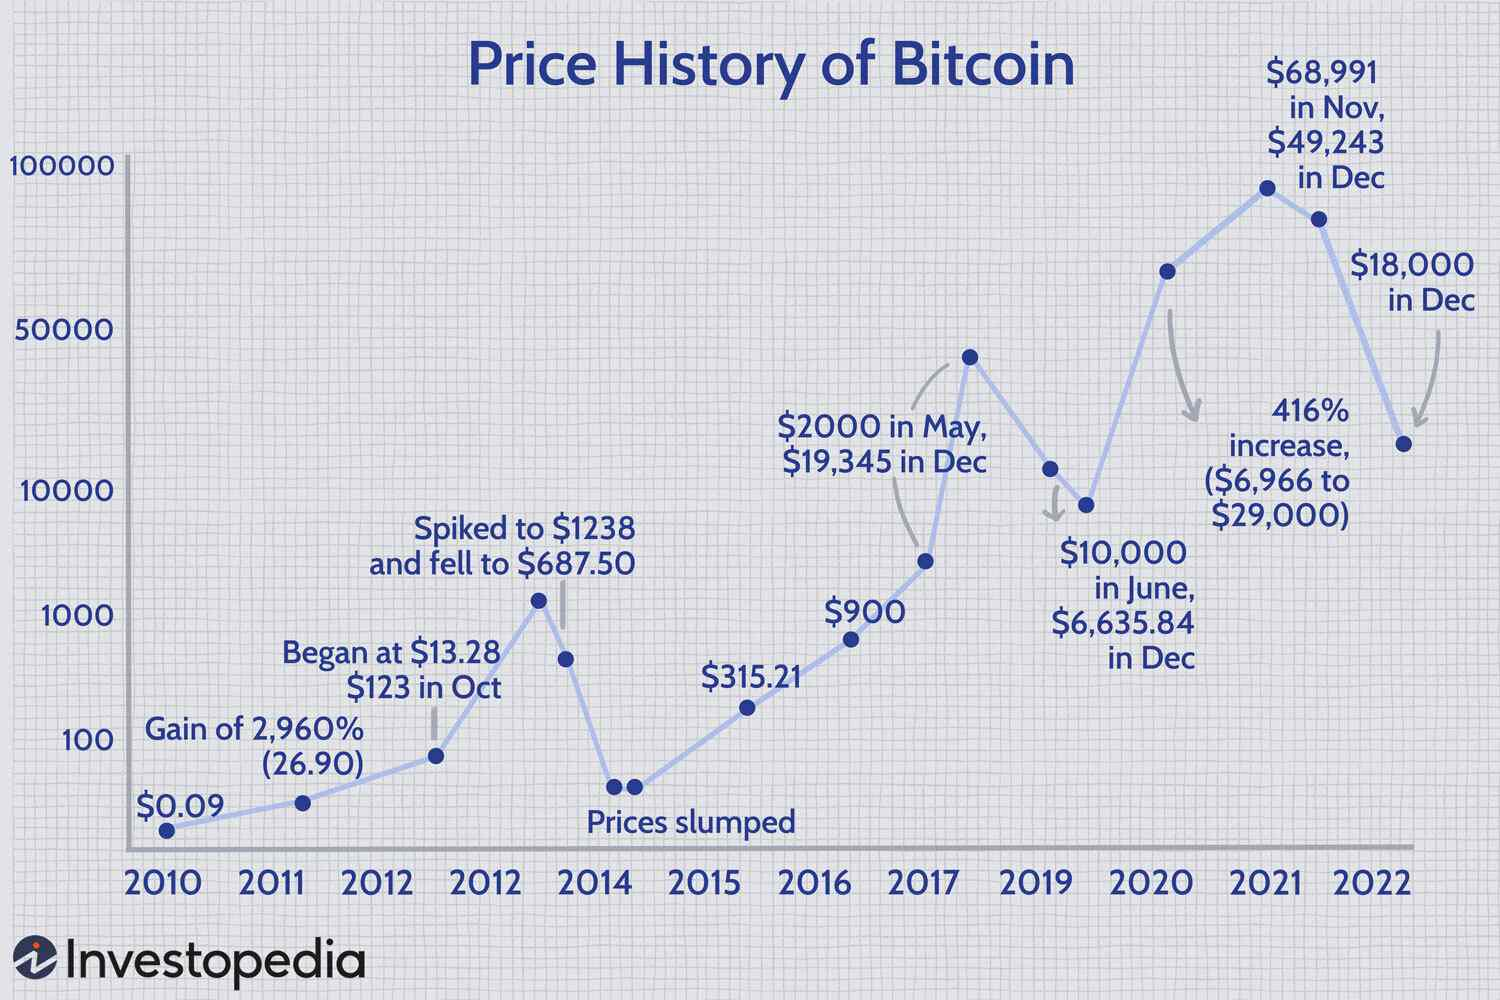
\includegraphics[scale=0.25]{Fig1.jpg}
\caption{Bitcoin Price Trend Overtime.}
\citep{noauthor_bitcoins_nodate}
\end{figure}



\subsection{Market Dynamics and Behavior}
Numerous internal and extrinsic factors, as well as market conditions, have an impact on Bitcoin's price dynamics. Unlike conventional financial assets, Bitcoin's valuation is not determined by cash flows, dividends, or interest payments. Alternatively, it is frequently compared to commodities like gold, acting as a store of value or "digital gold" \citep{DBLP:conf/ecis/GlaserZHW14}.
\smallskip

%%% ----------------------------------------------------------------------
Several factors impact Bitcoin's price:
\smallskip

%%% ----------------------------------------------------------------------
\textbf{Supply and Demand:} The total number of Bitcoin coins in circulation is 21 million. Given the shortage and rising demand, particularly from institutional investors, which can then lead to an overall price surge. \citep{DBLP:journals/ijecommerce/PolasikPWKL15}

\smallskip

\textbf{Regulatory News:} The price of Bitcoin can be significantly impacted by governmental rules or simply by the prospect of upcoming regulations. For instance, price reductions have typically been precipitated by regulatory crackdowns in nations like China \citep{feng_informed_2018}.

\smallskip

\textbf{Technological Changes and Innovations:} Technological developments in the blockchain industry or scaling solutions like the Lightning Network might affect investor sentiment and the price of Bitcoin. \citep{easley_mining_2019}

\smallskip

\textbf{Macroeconomic factors:} It can affect the price of decentralized assets like Bitcoin by increasing their allure. These factors include economic downturns, inflation rates, and political unrest. \citep{urquhart_inefficiency_2016}.

\smallskip

Markets for bitcoin are notorious for their high volatility. Its speculative nature, restricted liquidity, regulatory news, and macroeconomic factors might be blamed for this volatility. Furthermore, the actions of Bitcoin traders, particularly those motivated by herd behavior, worsen this volatility. \citep{bouri_hedge_2017}.

\goodbreak

\section{Machine Learning in Financial Computing}
\goodbreak

\subsection{Applications and Techniques:}

Over the past ten years, \gls{ml} has significantly advanced in the field of financial computing. Its uses are many, using sophisticated algorithms to inform choices, forecast market movements, spot fraud, and more.

\smallskip

\textbf{Portfolio Management (Robo-Advisors):}

The asset portfolios of customers are automatically allocated, managed, and optimized by robo-advisors using ML approaches in accordance with their unique preferences and goals. \gls{ml} models can optimize asset allocation more effectively than conventional techniques by analyzing enormous volumes of data \citep{goldstein_investor_2017}.

\smallskip

\textbf{Algorithmic Trading:}

High-frequency trading companies use ML algorithms to forecast price fluctuations on a millisecond time scale. These forecasts are based on massive databases, which also include order books, trading volumes, and even news items. Deep learning and neural networks have both proven extremely useful in this domain. \citep{DBLP:journals/cacm/TreleavenGL13}

\smallskip

\textbf{Credit Scoring:} 

Conventional credit scoring techniques frequently use manual procedures and standards based on rules. These models can be improved by \gls{ml}, which analyses a wider variety of data (including non-traditional data) and more accurately predicts the likelihood of defaults \citep{DBLP:journals/eor/LessmannBST15}.

\smallskip

\textbf{Fraud Detection:} 

\gls{ml} models can be taught to find patterns linked to fraudulent transactions. These algorithms can adapt and identify novel, previously unidentified types of fraud by continuously learning from fresh transactions \citep{10.1214/ss/1042727940}.

\goodbreak



\textbf{Risk management:} 

\gls{ml} can help, especially with complex financial products, in comprehending and managing risk. \gls{ml} models can offer more precise risk evaluations and even forecast probable market downturns by examining market conditions and historical data \citep{DBLP:journals/eswa/YehYT09}.

\begin{table}[H]
\centering
\begin{tabular}{|l|l|p{5cm}|}
\hline
\textbf{Applications} & \textbf{Tree-based Ensembles} & \textbf{Deep Learning Models} \\
\hline
Credit Scoring & Widely used & Emerging use \\
\hline
Fraud Detection & Commonly used & Widely used with neural networks \\
\hline
Algorithmic Trading & Used & More common with time-series data \\
\hline
Portfolio Management & Used & Emerging use
with reinforcement Learning \\
\hline
Risk Management & Widely used & Emerging use \\
\hline
\end{tabular}
\caption{Applications of Tree-based Ensembles and Deep Learning Models in Finance}
\citep{ravi2015survey}
\label{table:applications_comparison}
\end{table}

\goodbreak

\subsection{Opportunities and Challenges:}

\smallskip

Although ML has tremendous prospects for financial computing, it also poses difficulties:

\textbf{Data Quantity and Availability:}
 The effectiveness of ML models is strongly influenced by the quality and quantity of accessible data. When training robust models, financial institutions may struggle with inconsistent, missing, or unstructured data \citep{DBLP:journals/mansci/BaesensSMV03}.

\smallskip
 
\textbf{Interpretability: }
A lot of sophisticated ML models, particularly deep learning models, lack interpretability. The "black-box" character of some ML models raises questions in a field where decisions might have large financial repercussions \citep{DBLP:conf/kdd/Ribeiro0G16}.

\smallskip

\textbf{Overfitting:} 
There is a chance that ML models will become overly reliant on previous data, which will limit their ability to adapt to novel, unforeseen market conditions. Decisions made as a result of overfitting may not be the best ones \citep{DBLP:journals/jcisd/HawkinsBM03}.

\smallskip

However, these difficulties also present chances:

\smallskip

\textbf{Data engineering Solutions:} It can be used to ensure consistent, high-quality data for training, hence addressing the problem of poor data quality (Wang  Strong, 1996).

\smallskip

\textbf{Explainable \gls{ai}:} There is rising interest in creating sophisticated models that can also be understood. To increase the transparency of ML models, explainable \gls{ai}  techniques have been developed \citep{doshivelez2017rigorous}.

\smallskip

\textbf{Regularization Techniques:} It can be used to prevent overfitting and make sure that models generalize properly to fresh data \citep{10.1145/1015330.1015435}.

\goodbreak
\section{Tree-based Ensembles in Predictive Modeling}
\smallskip

%%% ----------------------------------------------------------------------
\goodbreak

\subsection{Random Forest in Finance}


In finance, the ensemble learning technique Random Forest can be applied to both classification and regression applications. To create more reliable forecasts, it mixes different decision trees \citep{breiman_random_2001}.

\textbf{Stock Price Prediction:} Random Forest has been used to forecast stock price changes, and many tests have found it to be highly accurate \citep{liaw2002classification}.

\textbf{Credit Risk Assessment:} The model has also been employed to assess borrowers' creditworthiness \citep{DBLP:conf/kdd/ChenG16}.

\goodbreak

\subsection{Other Ensemble Methods:}

Other popular tree-based ensemble techniques in the finance industry include:

\textbf{Gradient Boosting:} According to \cite{4a848dd1-54e3-3c3c-83c3-04977ded2e71}, this technique creates trees one at a time, fixing the mistakes of the preceding ones.

\textbf{AdaBoost:} It is a different boosting technique that is focused on difficult-to-predict situations \citep{DBLP:conf/icml/FreundS96}.

\textbf{XGBoost:} It is a gradient boosting extension that is renowned for its computational effectiveness \citep{DBLP:conf/kdd/ChenG16}.



\subsection{Performance Metrics:} 

\goodbreak

 The validation of a model's effectiveness is, as much as it is the modeling itself, an important factor for prediction models that are especially applicable to finance applications. A set of performance metrics shall be used to determine the reliability and precision of the model. These measures provide a quantitative assessment of the model's assumptions, as opposed to its actual results.


\textbf{Accuracy:}   Accuracy calculates the proportion of accurately predicted instances to all instances, making it the most simple metric. Accuracy can be deceptive, even though it offers a preliminary assessment of model performance, particularly in unbalanced datasets where one class is disproportionately overrepresented  \citep{M2015ARO}.

\[ \text{Accuracy} = \frac{\text{Number of correct predictions}}{\text{Total number of predictions}} \]

\textbf{Precision and Recall:} It rates the precision of correct predictions. An algorithm with great precision will have returned significantly more relevant results than irrelevant ones. and Recall calculates what percentage of all relevant instances were actually retrieved. When the cost of missing a favorable instance is high, it is essential.
 \citep{DBLP:journals/corr/abs-2010-16061}.

\[ \text{Precision} = \frac{\text{True Positives}}{\text{True Positives} + \text{False Positives}} \]

\[ \text{Recall} = \frac{\text{True Positives}}{\text{True Positives} + \text{False Negatives}} \]

\textbf{F1 Score:} The F1 Score is a harmonic average of precision and recall that mediates the balance between precision and recall. F1 scores closer to one mean better precision and performance balance\citep{DBLP:journals/ipm/SokolovaL09}.

\[ F1 = 2 \times \frac{\text{Precision} \times \text{Recall}}{\text{Precision} + \text{Recall}} \]


\textbf{Root Mean Square Error(RMSE):}

For regression problems or financial forecasting, \gls{rmse} measures how accurately the model predicts the outcome. This gives an idea of the size of the error between the predicted and observed values.

\[ \text{RMSE} = \sqrt{\frac{1}{n} \sum_{i=1}^{n} (y_i - \hat{y}_i)^2} \]

\textbf{\gls{auc}:}
 In the case of classification problems, the \gls{auc} of the receiver operating characteristic \gls{roc} curve is an essential metric. The ability of the model to distinguish between positive and negative classes is illustrated. A more refined model is implied by an \gls{auc} closer to 1.

\goodbreak
\section{Deep Learning Models for Trading Analysis}
\smallskip

%%% ----------------------------------------------------------------------
\subsection{LSTM and Time Series Prediction}
\goodbreak

Recurrent Neural Networks (RNN) Long Short-Term Memory (LSTM) networks are crucial for forecasting time-series data. They have a wide range of uses in the financial markets, particularly for predicting price movements in the trading of bitcoins:

\textbf{Application In Bitcoin Trading:} According to \cite{DBLP:conf/nips/SutskeverVL14}, LSTM models are used to identify long-term dependencies and sequential information in Bitcoin price data. This helps to make precise predictions.


\textbf{Strengths and Limitations:} While LSTMs provide a sophisticated understanding of time-dependent data structures, their usefulness may be limited by the processing requirements and difficult hyperparameter tuning \citep{DBLP:journals/corr/ChungGCB14}.


\textbf{Comparison with Other Models:} According to \cite{DBLP:journals/neco/GersSC00}, LSTM frequently offers greater forecasting performance in erratic markets like Bitcoin. This is demonstrated by a comparison between LSTM and conventional time-series models like ARIMA.

\subsection{Modern Tools and Innovations} 

\goodbreak

With new developments, the use of deep learning in Bitcoin trading analysis continues to advance:

\textbf{\gls{drl}: }According to \cite{DBLP:journals/nature/MnihKSRVBGRFOPB15}, DRL has become a potent tool for optimizing trading tactics in Bitcoin markets by dynamically adjusting to market changes.

\textbf{Pre-trained Models:} Using pre-trained models for sentiment research, such as BERT, has revealed fresh information about market patterns in the bitcoin industry \citep{DBLP:journals/corr/abs-1810-04805}.

\textbf{Tools and Frameworks:} In the context of Bitcoin trading, frameworks like TensorFlow and PyTorch have made deep learning model deployment and experimentation more accessible \citep{DBLP:journals/corr/AbadiABBCCCDDDG16}\citep{DBLP:journals/corr/abs-1912-01703}.

\goodbreak
\section{Economic and Statistical Metrics for Evaluation}
\smallskip

%%% ----------------------------------------------------------------------
\subsection{Traditional Statistical Metrics}
\smallskip

Common metrics for measuring prediction mistakes, particularly in continuous forecasts like price trends, include mean squared error (MSE) and root mean square error (RMSE) \citep{hyndman_another_2006}.

\textbf{Accuracy, Precision, Recall, and F1-Score:} When the prediction job is stated as categorization, such as predicting upward or downward market movements, accuracy, precision, recall, and F1-Score metrics can be used \citep{DBLP:journals/ipm/SokolovaL09}.

\textbf{Time Series Specific Metrics:} Metrics Particular to Time Series: According to\citep{9f5faea9a4884eff9665c32105db424f}, time series forecasting is particularly relevant to specialised metrics like Mean Absolute Percentage Error (MAPE).

\subsection{Economical Significance}
\smallskip

\textbf{Profit and Loss Evaluation:} Metrics that measure the financial gains from implementing the model's predictions in actual trading scenarios.

\textbf{Metrics Based on Utility:} 
Taking into account the risk against benefit trade-off in relation to financial trading and investing \citep{danielsson_model_2016}.

\textbf{Market Impact Assessment:} Analysing the models in light of possible market effects including those on volatility and liquidity.

\subsection{Comparison Across Models}
\smallskip

\textbf{Statistical Tests for Comparing Models:} Methods for statistically comparing the performance of several models to identify significant differences, such as the Diebold-Mariano test \citep{doi:10.1080/07350015.1995.10524599}.

\textbf{Economic Value of Predictive Accuracy:} Models are evaluated not only for their statistical significance but also for their usefulness to traders and investors \citep{26d24c7c-b91e-306e-b000-d5246fb6c3cb}.

\goodbreak
\section{Summary of the Literature Gap}
\goodbreak

\subsection{Lack of Comprehensive Comparative Studies}
\goodbreak

There may be a dearth of thorough studies that systematically evaluate deep learning models like LSTM with tree-based ensemble approaches like Random Forest for forecasting fluctuations in the price of bitcoin \citep{8631923}.

Numerous studies might concentrate on one method over another, although direct comparisons might be uncommon or limited to certain data sets or periods.

\subsection{Inconsistent Evaluation Metrics}

Drawing findings that are consistent across studies may be challenging due to the wide variations in the measures employed to assess the performance of these models \citep{doi:10.1198/016214506000001437}.
\smallskip

It's possible that there isn't enough standardization when taking into account both economic and statistical significance, which results in inconsistent findings.

\subsection{Emerging Market Behavior}

Since they are very young, cryptocurrencies like Bitcoin and others act differently from conventional financial instruments. According to \citet{nadarajah2017inefficiency}, this dynamic may call for novel predictive modeling approaches and techniques that haven't received much attention in the literature so far.

There may be a gap in the literature due to the volatility and unpredictable nature of cryptocurrencies, which may present particular problems that call for particular solutions.

\subsection{Ethical and Regulatory Considerations}

Ethics-related issues, such as the possible effects of predictive models on market stability and integrity, may not be adequately addressed by existing research.

The impact of regulatory compliance on the creation and application of these predictive models in the trading area may also go unexplored \citep{arner2015evolution}.






   


\def\baselinestretch{1.66}
\medskip


%%% ----------------------------------------------------------------------

% ------------------------------------------------------------------------
% -*-TeX-*- -*-Hard-*- Smart Wrapping
% ------------------------------------------------------------------------
\def\baselinestretch{1}

\chapter{Methodology Design}

\def\baselinestretch{1.44}

%%% ----------------------------------------------------------------------

This chapter presents the methodical technique used in this work to analyze and contrast the statistical and economic significance of deep learning models and tree-based ensembles in predicting Bitcoin trading directions. 
   
\smallskip

%%% ----------------------------------------------------------------------
\goodbreak
\section{Research Design}
\goodbreak

\subsection{Research Paradigm }

The positivist paradigm, which this research largely adheres to, emphasizes objective measurements and the empirical examination of data in order to identify patterns and draw reliable conclusions \citep{alma9924678548402466}. This paradigm offers the best basis for the investigation given the numerical nature of trade data and the empirical aspects of machine learning.

\subsection{Research Approach}

The study uses a quantitative research methodology. Given that the study used historical Bitcoin trading data and computational models, this is characterized by the use of numerical data and quantitative analysis \citep{creswell2014research}.

\subsection{Data Collection}

For this study, historical Bitcoin trade data that included daily trading metrics including prices, volume, and other trading indicators was gathered.

The dataset was obtained from (for example," Yahoo Finance") and covered the period from (01/01/2021) to (05/07/2023).

\subsection{Data preparation}

The dataset received extensive preprocessing to guarantee the correctness and dependability of the models. This comprised:

-	dealing with missing values.

-	detection and correction of outliers.

-	Feature engineering: To gain insight into daily percentage changes in closing prices, 
variables like "Return" were computed.

-	Data normalization: It is crucial, especially for LSTM and other deep learning models.

\subsection{Model Development }

There were two primary models chosen:

\textbf{Tree-based Ensemble:} To be more precise, the Random Forest Classifier was used to forecast the movement of the Bitcoin price.

\textbf{Deep Learning Model:} To capture the sequential character of the trading data, the LSTM (Long Short-Term Memory) network, which is particularly well suited for time series prediction, was used as the deep learning model.

Both models were evaluated on a subset of the data (i.e., 70 percent of the dataset). which is Train data and then the rest 30 percent of the dataset is known as the Test dataset.

\subsection{Model Evaluation}

Several performance criteria were taken into account in order to compare the two models
Statistical and economic significance:

-	Accuracy

-	Recall, precision, and F1 score

-	RMSE, or Root Mean Square Error

-	economic indicators, such as possible gains or losses from trading plans based on model predictions.

\medskip

\section{Data Collection and Pre-processing}

The caliber and type of data are crucial in the fields of machine learning and deep learning. This part explores the sources of the data, the standards used to choose it, and the techniques used to guarantee its accuracy for the study.

\subsection{Data Sources}

Yahoo Finance is a credible platform that offers historical data on cryptocurrency prices, trading volumes, and other important market indicators. This platform provided the primary data for this study. Due to its extensive data coverage, regular updates, and general acceptance in financial research on cryptocurrencies, this platform was selected \citep{smith2016predictive}.

\subsection{Selection Criteria}

For the data, the following standards were established:

\textbf{Timeframe:} The data spans ["from January 1, 2021, to July 05, 2023"], guaranteeing a rich set of historical data while also capturing current market movements.

\textbf{Frequency:} Daily closing prices were employed. This frequency was chosen to capture large price changes while reducing intraday volatility.

\textbf{Data Completeness:} Only data sets without any missing values for the designated indicators were taken into consideration.

\subsection{Preprocessing Steps}

Several preparation processes were used because raw financial data frequently contains imperfections:

-	\textbf{Cleaning}: Anomalies, outliers, and missing values were checked in the initial data. 
Imputation was done using linear interpolation in cases where there were missing data points.

-	\textbf{Normalisation:} The data was normalized, often scaling the values between 0 and 1, to make the training process more stable and quicker, especially for the LSTM model \citep{Goodfellow-et-al-2016}.

-	\textbf{Feature Engineering:} New features, including technical indicators, moving averages, and historical volatilities, were derived from the current data to give the models more contextual information.

-	\textbf{Data Splitting:} The dataset was split into training (70 percent) and testing (30 percent) sets in order to assess the performance of the models.

\goodbreak

\section{Random Forest Model}

During training, many decision trees are built using the ensemble learning technique known as random forests, which then produce the majority class for classification or the average prediction for regression. Because individual tree forecasts are averaged, random forests have the advantage of being somewhat resistant to overfitting and being able to model non-linear decision boundaries and feature interactions.

\subsection{Model Development}

The steps taken to create the Random Forest model for forecasting Bitcoin price movement are described in this subsection:

\textbf{Data Preprocessing:}

-	The dataset, which includes the closing prices for Bitcoin each day, has been loaded.

-	The calculated 'Return' shows the percentage change in the closing price from the previous day.

-	In order to indicate whether the return is positive (1) or not (0), a binary target variable is established.

\textbf{Feature Selection:}

-	The feature matrix, X, is created by removing unnecessary columns from the dataset, including "Date," "Return," and "Close."

\textbf{Data Splitting:}

-	The dataset is divided into training windows of various sizes, including 50 percent, 60 percent, 70 percent, and 80 percent. Tests are conducted using the remaining data. This configuration looks at the effects of changing the training window on the model's performance.

-	In order to maintain the data's temporal order during cross-validation, Timeseries Split is used on the training set of data.

\textbf{Model Training:}

-	One hundred trees are used to initialize a RandomForestClassifier.

-	The model is trained on the training fold and validated on the validation fold during cross-validation. This procedure is repeated for each fold, enabling an evaluation of the model's performance and stability over time.

\subsection{Model Evaluation}

This section assesses how well the Random Forest model performs:

\textbf{Test Set Evaluation:}

-	The model is retrained on the complete training set following cross-validation, and it is then assessed on the test set. This is an estimate of the model's performance on brand-new, untested data.

\textbf{Performance metrics:}

-	Between the anticipated probabilities and the actual binary outcomes, the Root Mean Square Error (RMSE) is determined. The model's prediction error is estimated by RMSE.

-	For both positive and negative classes, classification reports are created that include metrics like precision, recall, and the F1-score. This clarifies how well the algorithm can forecast both price increases and declines.

\textbf{Trading Strategy Evaluation:}

-	It uses a "Long or Short" trading approach. Buying when the model predicts a price increase and selling short when a reduction is anticipated is simulated in this way.

-	In order to illustrate the economic importance of the model's predictions under various training circumstances, the cumulative profit/loss over time, depending on this technique, is plotted for each training window size.

\textbf{Visualizations:}

-	The cumulative profit/loss curve and estimated return probabilities are displayed on graphs. This gives a visual depiction of the forecasts and economic impact of the model.

\goodbreak

\section{LSTM (Deep Learning) Model}

Long Short-Term Memory (LSTM) is a special sort of Recurrent Neural Network (RNN). RNNs use loops to store information rather than the independent processing of inputs found in traditional neural networks \citep{Hochreiter1997LongSM}. Standard RNNs, on the other hand, frequently struggle with long-term dependencies because of problems like vanishing or ballooning gradients. With their unique architecture, LSTMs efficiently handle these issues.

Why Do we use LSTM for time series forecasting?

Data points in a time series are sequential and exhibit a temporal association. Because they are designed specifically to identify patterns over time, LSTMs are well-suited for applications where the sequence and order of data points are important, such as stock price prediction or weather forecasting \citep{DBLP:conf/nips/SutskeverVL14}.

For instance, when anticipating Bitcoin prices, a variety of events from days, weeks, or even months ago may have an impact on the price today. For such forecasting tasks, LSTMs are a great option since they may be able to identify and record these long-term dependencies and trends \citep{moghar2020stock}.

\subsection{Model Development }

\textbf{Data Preparation:}

The data is normalized before training to ensure that all input features scale equally, often between 0 and 1. The training process is aided by such scaling, making it more effective and stable.

\textbf{Model Architecture:}

In this situation, the LSTM model consists of:

-	\textbf{Input LSTM Layer:} Bitcoin price sequences are processed by the input LSTM layer, which then produces another sequence suitable for the output LSTM or Dense layer \citep{Hochreiter1997LongSM}.

-	\textbf{Dense Layer:} This layer of a typical neural network connects every input node to every output node. It analyses the output sequence from the LSTM layer above and outputs a single value, the projected price.

The backpropagation over time iterative approach is used to train the model on previous Bitcoin data.

\subsection{Model Evaluation:}

\textbf{Trading Strategy Implementation:}

The model's predictions are used to develop a "long or short" trading strategy:

-	If the model foresees an increase in price (bullish sentiment), a long position is taken, which implies buying the asset.

-	In contrast, a short position is opened if a downward movement is anticipated (bearish attitude), wagering against the asset in anticipation of a decline in value.

Although this technique provides a basis for review, it is a simplification and might not accurately reflect the nuances of real-world trading.

\textbf{Visualizing Predictions}: 
To understand the model's performance, forecasts and prices are compared. Such a visual depiction makes it easy to distinguish between the model's correct predictions and its errors.

\textbf{Final Portfolio Value:} Using the "long or short" technique, the final portfolio value may be calculated. In a fictitious trading scenario, this number serves as a tangible criterion to assess the model's forecasting skill.

\textbf{Training Window Size Impact:} The model's performance is also evaluated using a range of historical data (such as 60 percent, 70 percent, etc.). Such an assessment aids in calculating the ideal amount of historical data needed for the best results.

\textbf{Insights:}

With their innate design, understanding LSTM models excel at forecasting time series data, such as Bitcoin values. There are a couple of limitations, though:

-	Many of the factors that affect financial markets may not be present in historical pricing data.

-	Although LSTMs are capable of detecting long-term dependencies, they are not perfect. It is crucial to regularly assess models and update them with fresh data \citep{moghar2020stock}.

\goodbreak



\subsection{Data Load and PreProcessing}

A structured dataset is loaded with Bitcoin trading data from a CSV file. To simplify time-based operations, the dataset's 'Date' items are transformed into a standardized date-time format. After that, the data is chronologically arranged. The daily percentage change in the closing prices of Bitcoin is calculated and displayed in a new column named "Return." For trading strategy implementation, this "Return" is crucial. The retrieved Bitcoin closing values are then scaled between 0 and 1. For deep learning models like LSTMs in particular, this scaling is an essential preprocessing step that makes sure the model converges more quickly and performs better.

\subsection{LSTM Model With Adjusted (No of Days)}

\textbf{Model Training and Prediction:}

- Based on a predetermined number of days, the data is divided into training and validation datasets.

- On the training dataset, the LSTM model is trained. It gains the ability to predict, using today's price, the closing price for the following day.

- The model predicts the closing prices on the validation dataset following training.

\textbf{Trading Strategy Implementation:}

- Based on the model's predictions, a "long or short" trading strategy is created.

- If the model predicts that the price will be higher than it is today on the next day, a "long" position is taken, and if it predicts that the price will be lower, a "short" position is taken.

- Daily changes are made to the beginning capital depending on the real return to reflect any gains or losses from the approach.


\section{Comparative Analysis Method}

\goodbreak

Long Short-Term Memory (LSTM) networks, a sort of deep learning model, and the Random Forest, a tree-based ensemble method, were both used to predict Bitcoin prices. We can systematically analyze these two approaches using comparative analysis to ascertain their relative merits and shortcomings in the context of our particular issue.

\subsection{Data and Metrics Selection: }

\textbf{Data:} The same Bitcoin price dataset was used to train and assess both the LSTM and the Random Forest models. This guarantees that the comparison is solely focused on the capabilities of the models and is unaffected by any data inconsistencies.

\textbf{Metrics:} We mainly concentrated on the models' capacity to make profits using a trading strategy for our specific problem of predicting Bitcoin prices. The accuracy of the models' predictions could also be evaluated using other metrics, such as Mean Squared Error (MSE) \citep{DBLP:books/lib/HastieTF09}.

\subsection{Analysis Process}

\textbf{LSTM (Deep Learning Model):}


\textbf{Model Complexity:} Recurrent neural networks, such as LSTMs, are intrinsically complicated and computationally demanding. Their memory cells, which can record long-term dependencies, make them particularly skilled at managing time series data.

\textbf{Training Time:} Training an LSTM may be time-consuming and frequently calls for specialized gear like GPUs, especially when dealing with large amounts of data.

\textbf{Performance:} Non-linear patterns in the data may be captured by LSTMs that simpler models may miss.

\textbf{Random Forest (Ensemble Model):}


\textbf{Model Complexity:} Random Forests are ensemble techniques that are based on trees. Although each tree is straightforward on its own, integrating other trees makes the model more complex.

\textbf{Training Time:} Usually quicker than training deep learning models like LSTMs, but with huge datasets or a lot of trees, it might still take a while.

\textbf{Performance:} Random Forests have a reputation for being highly accurate and capable of handling non-linear data patterns. Additionally, they convey feature importance by revealing which traits have the greatest impact on predictions \citep{breiman_random_2001}.

\subsection{Insights and Interpretations:}

Following a thorough investigation, the following conclusions can be drawn:


\textbf{Trading Strategy Performance:} In our particular situation, the main objective was to maximize profits using a trading technique. To assess both models' applicability in the actual world, they were included in trading strategies.


\textbf{Model Suitability:} LSTMs are capable, however for some datasets, they may be overkill. It could be desirable if the Random Forest can achieve comparable performance with less complexity and quicker training timeframes.


\textbf{Infrastructure and Resources:} More computational resources are often needed for LSTMs. Random Forest might be a better option if resources are few.

\textbf{Insights:}

Both Random Forest and LSTM offer particular advantages. The capacity to capture long-term dependencies in time series data may be where LSTMs shine, but Random Forests combine accuracy, interpretability, and minimal processing requirements. Based on the individual issue, the available resources, and the intended results, one should select one over the other (Demsar, 2006).

\medskip

\section{Summary} 

We set out on a thorough methodological journey to forecast Bitcoin values in this chapter, contrasting deep learning models with ensembles that are built using trees. Here is a brief summary:

\textbf{1. Research Design:}

The research, which had its roots in the positivist paradigm, placed a strong emphasis on the objective, empirical analysis of trade data to find trends and conclusions.

Given that the study was mostly based on historical Bitcoin trading data, a quantitative research methodology was employed, utilizing numerical data and analysis methodologies.

\textbf{2.Data Collection and Preprocessing:}

The foundation of this study was historical Bitcoin trade data, which comprised a wide range of trading parameters. After gathering the data, the following preprocessing procedures were used:

-	cleaning, which involved fixing abnormalities, outliers, and missing values.

-	Normalization is done largely to keep the training process stable.

-	Additional contextual features were extracted using feature engineering.

-	Splitting data for training and testing.

\textbf{3. Model Exploration:}

\textbf{Random Forest:}

Random Forest, a method of group learning, was used. During training, it builds a number of decision trees and generates an average result. It is renowned for its capacity to simulate non-linear data and provide perceptions of key elements.

\textbf{LSTM (Deep Learning Model):}

A subgroup of RNNs called LSTMs was first developed. They are skilled at managing time series data thanks to their memory cells, which makes them suitable for forecasting data points that are sequential and display temporal correlations, such as Bitcoin values.

\textbf{4. Comparative analysis:}

The LSTM and Random Forest models were compared side by side. In this analysis, different aspects of both models were examined, such as:

-	Model Complacency.

-	Training time.

-	Performance.

-	Real-world Applicability

It was concluded that while Random Forests offer a blend of accuracy, interpretability, and efficiency, LSTMs excel at capturing long-term dependencies. The decision between the two is based on the requirements of the particular project, the computational resources at hand, and the intended results.

This chapter essentially offered a thorough framework for forecasting Bitcoin prices, emphasizing the distinctive advantages and potential drawbacks of both LSTM and Random Forest models. It offers scientific rigor and useful insights, serving as a road map for anyone wishing to explore the complex world of Bitcoin price prediction.

   

\def\baselinestretch{1.66}
\medskip

%%% ----------------------------------------------------------------------

% ------------------------------------------------------------------------
% -*-TeX-*- -*-Hard-*- Smart Wrapping
% ------------------------------------------------------------------------
\def\baselinestretch{1}

\chapter{Results}

\def\baselinestretch{1.44}

%%% ----------------------------------------------------------------------
The Results section offers a thorough overview of the conclusions drawn from our methodology, with a special emphasis on the ability of the Random Forest model to forecast changes in the price of bitcoin.

\smallskip

%%% ----------------------------------------------------------------------
\goodbreak
\section{Random Forest Performance}
\goodbreak

A well-known ensemble learning technique called Random Forest combines predictions from various decision trees to provide a consolidated result. It is a great tool for predicting Bitcoin values due to its complex capacity to unravel non-linear patterns in datasets.


\subsection{Model Training and Validation:}

Time Series Cross-Validation (TSCV) was used to train and validate the model. This method is specifically designed for time series data, such as Bitcoin price data, where the sequential nature of data points is crucial. The model was tested over five different training-validation windows to guarantee robustness.

A Multiple Training Windows Approach was also used to investigate the effect of training window size on model performance. The size of the training window can be quite important. More historical data is available with a bigger training window, which may help to identify long-term trends. A smaller window, though, might be more responsive to current developments. The model was trained using three different lengths of historical data: 50 percent, 60 percent, and 70 percent of the dataset, in order to determine the best window size for our data.

\subsection{Performance Metrics across Validation Windows:}

-	\textbf{Root Mean Squared Error (RMSE): }

\begin{figure}[H]
\centering
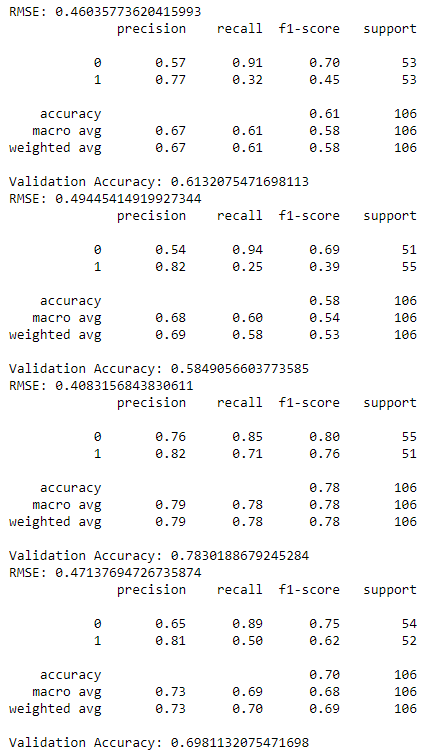
\includegraphics[scale=0.85]{fig2.jpg}
\end{figure}

\begin{figure}[H]
\centering
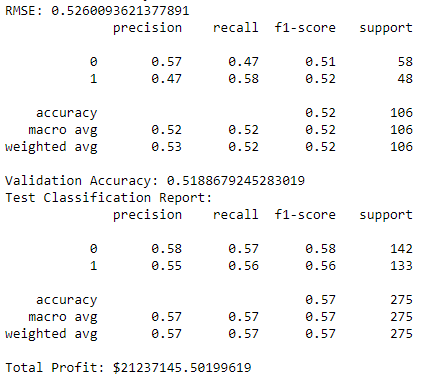
\includegraphics[scale=0.85]{fig3.jpg}
\end{figure}

RMSE is a metric for gauging how well a model predicts a result. Lower RMSE values are preferred since they show better data fit. The observed RMSE values were 0.460, 0.494, 0.408, 0.471, and 0.526 for the five validation windows. The variation in RMSE across windows highlights the underlying volatility of Bitcoin values.

-	\textbf{Accuracy:} The ratio of successfully predicted instances to all instances is provided by this metric. Across the five validation windows, the model received accuracy scores of 61.32 percent, 58.49 percent, 78.30 percent, 69.81 percent,51.89 percent, and 57.00 percent, respectively. Given the unpredictability of cryptocurrency prices, these figures suggest a fair amount of fit.

-	\textbf{Precision:} Represents the proportion of accurate positive forecasts among all positive predictions. Precision for estimating price increase (1) ranged from 0.82 to 0.47 among the from 0 to 1 window.

-	\textbf{Recall:} Indicates the proportion of accurate positive forecasts among all real positives. The range of recall values for forecasting price increases was 0.25 to 0.94 among the 0 to 1 window.

-	\textbf{F1 Score:} The harmonic mean of recall and precision is the F1-score. A balanced performance was shown by F1-Scores for predicting price increases, which varied from 0.39 to 0.80 among the 0 to 1 window.


\medskip

\textbf{Performance in the Multiple Training Windows Approach Across Different Windows:}

\begin{figure}[H]
\centering
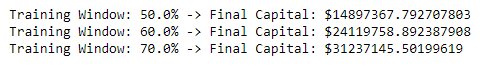
\includegraphics[scale=0.85]{fig4.jpg}
\end{figure}

-	\textbf{Training Window 50 percent:} Using half the dataset for training produced a final capital of about 14,897,367.79 Dollars, indicating a 4,897,367.79-dollar profit from an initial 10,000,000 Dollars.

-	\textbf{Training Window 60 percent:} The model technique resulted in a capital of about 24,119,758.89 Dollars, indicating a profit of about 14,119,758.89 Dollars, with a training window of 60 percent of the dataset.

-	\textbf{Training Window 70 percent:}  70 percent of the data was used for training, producing a capital of around 31,237,145.50 Dollars and a profit of about 21,237,145.50 Dollars.



\subsection{Visualization insights:}

Three useful visualizations were produced:

\textbf{1. Predicted Return Probabilities Over Time:} 

\begin{figure}[H]
\centering
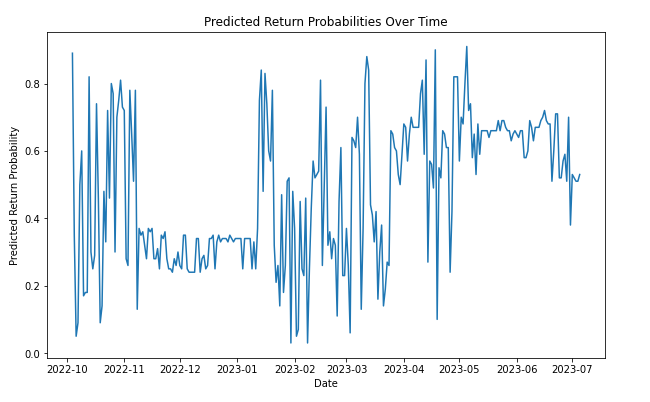
\includegraphics[scale=0.85]{fig5.jpg}
\caption{Predicted Return Probabilities Over Time}
\label{Predicted Return Probabilities Over Time}
\end{figure}

Figure 4.1 shows how expected return probabilities fluctuated during the test period.

This graph illustrates how confidently the model makes predictions over time. A higher probability denotes a more fervent expectation that the price will increase the following day.

\textbf{2.	Cumulative Profit/Loss Over Time:}

\begin{figure}[H]
\centering
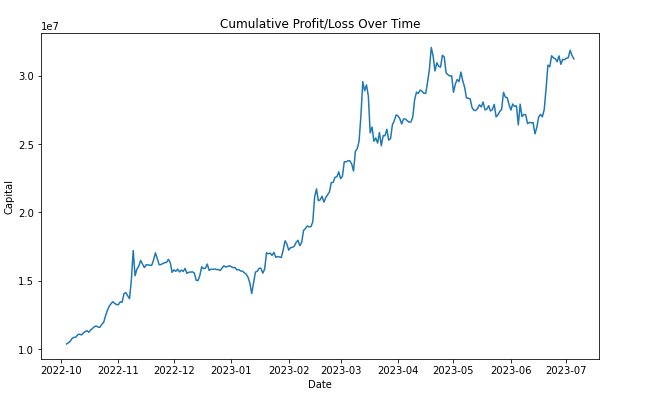
\includegraphics[scale=0.85]{fig6.jpg}
\caption{Cumulative Profit/Loss Over Time}
\label{Cumulative Profit/Loss Over Time}
\end{figure}

Figure 4.2 shows the cumulative profit/loss trajectory when using the trading suggestions from the algorithm.

This visualization illustrates the overall financial effects of using the trading strategy suggested by the model. The profitability of the strategy is indicated by a steadily increasing trend.

\textbf{3.	Final Capital vs. Training Window Size:} 


\begin{figure}[H]
\centering
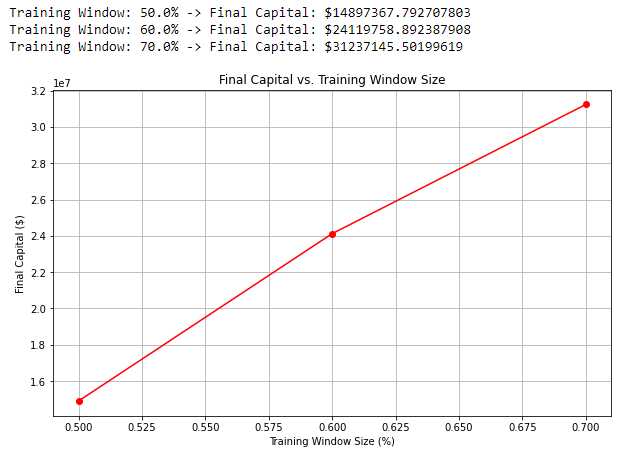
\includegraphics[scale=0.85]{fig7.jpg}
\caption{Final Capital vs. Training Window Size}
\label{Final Capital vs. Training Window Size}
\end{figure}
Figure 4.3 shows the connection between the dimensions of the training windows and the total capital gained. As seen, greater earnings result from a wider training window.

A plot juxtaposing the final capitals against the training window sizes was generated for a clearer understanding.

\subsection{Comparison of trading Strategies(Long or Cash)(Long or Short) In Random Forest}

\textbf{Model Performance: }
During cross-validation, the model's performance on several validation sets is presented. The model's accuracy, sensitivity, and harmonic mean of precision and recall are revealed through metrics like precision, recall, and f1-score.

\textbf{Results of a trading strategy:}

\textbf{Long or Cash Strategy}: With 10 million dollars in initial capital, the strategy generates a profit of about 13.21 million Dollars.

\textbf{Long or Short Strategy}: This strategy generates a higher profit of about 21.24 million dollars using the same initial cash.

\textbf{Visualization: }

A plot depicts the overall profit or loss for both techniques over time. Understanding the capital's growth trajectory and contrasting the performance of the two strategies over the test set is made easier thanks to this graphical representation.

\begin{figure}[H]
\centering
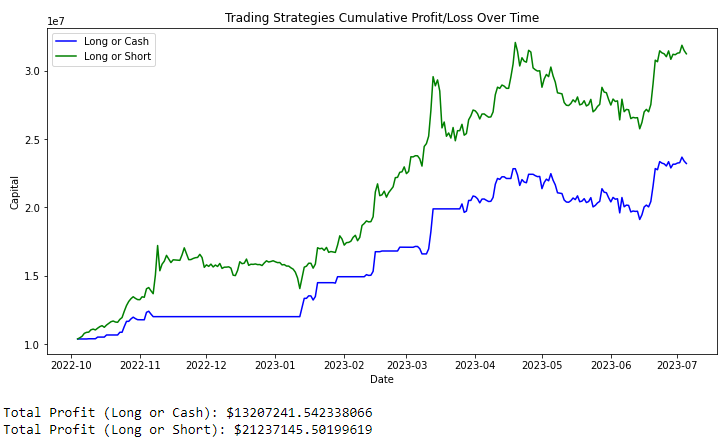
\includegraphics[scale=0.85]{fig8.jpg}
\caption{Comparison of trading Strategies(Long or Cash)(Long or Short) }
\label{Comparison of trading Strategies(Long or Cash)(Long or Short)}
\end{figure}

\subsection{Conclusion for Random Forest Performance:}

A few significant findings are shown when the Time Series Cross-Validation (TSCV) and Multiple Training Windows techniques:

\textbf{Model Robustness:} The Random Forest model produced profits consistently over a range of validation windows and training sizes.
Optimal Window Size: The best window size produced a profit of 70 percent, indicating that using more historical data can help project Bitcoin values.

\textbf{Economic Significance:} In addition to traditional performance measurements, the significant profits made highlight the model's useful applications for Bitcoin trading. Understanding the practical ramifications of these forecasts is essential in addition to the measurements. An overall profit of 21,237,145.50 Dollars was realized by applying a straightforward trading strategy based on the model's predictions on the validation set. This large number highlights the usefulness and potential profitability of utilizing the Random Forest model to anticipate Bitcoin trade.

\goodbreak
\section{LSTM Performance}
\goodbreak

Recurrent neural network (RNN) architecture's Long Short-Term Memory (LSTM) networks, a subtype, are lauded for their aptitude for identifying and understanding long sequences. Due to its suitability for time series forecasting, which calls for the detection of patterns in sequential data \citep{Hochreiter1997LongSM}. 

\subsection{Model Training and Validation:}

\textbf{Model Architecture:}

The LSTM model's architecture consisted of two LSTM layers, followed by a Dense layer. To guarantee sequential input for the following LSTM layer, the first 50 units of the LSTM layer were programmed to return sequences. It was intended for the terminal Dense layer to produce a single value that foretells the following data point in the series. The model used the Adam optimizer for optimization and Mean Squared Error as the loss function.

\textbf{Training Across Multiple Windows:}

Temporal patterns are frequently visible in financial data, especially time series data. To determine the ideal window size for prediction, the LSTM model in this study was trained on historical data spanning window sizes of 60 percent, 70 percent, 80 percent, and 90 percent of the training data.

\subsection{Performance Metrics Across Training Windows:}

\textbf{Model Training Iterations:} For optimization, each training window underwent several iterations. The step progress bar (example: [================ Depending on the size of the window, each iteration took different amounts of time; larger windows took longer because there was more data to process. For illustration:

60 percent of the training window was finished in 8 iterations.
70 percent of the training window was finished in 6 iterations.
80 percent of the training window was finished in 4 iterations.
90 percent of the training window was finished in 2 iterations.

\textbf{Trading Strategy: }

Following the prediction, a "long or short" trading strategy was implemented. A long position (asset purchase) was taken if the model indicated an upward trend (rising price). Conversely, a short position was taken (asset sold) if a downward movement (price drop) was anticipated.

\textbf{Test Set Evaluation: }

The model was retrained on the entire training set after identifying the ideal training window size, and it was then assessed on a different test set. After applying the "long or short" trading method to the test data, the total portfolio value was roughly 19,002,979.05 Dollars. This implies that, when used in trading, the forecasts of the LSTM model may yield large profits. Given an original investment of 10,000,000.00 Dollars, this predicts a profit of about 9,002,979.05 Dollars.

\subsection{Visualization Insights: }
Plotting the actual vs. expected Bitcoin prices was shown in a visualization. The model's capacity to forecast over time is shown visually, enabling a qualitative evaluation of the model's accuracy and dependability.


\begin{figure}[H]
\centering
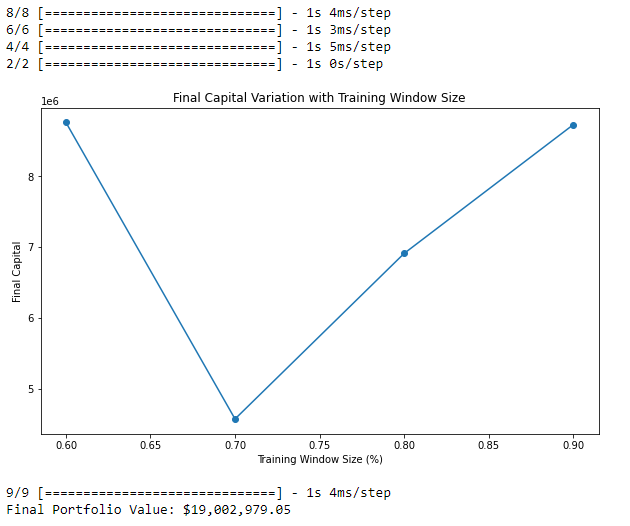
\includegraphics[scale=0.85]{fig9.jpg}
\caption{Final Capital Variation with Training Window Size}
\label{Final Capital Variation with Training Window Size}
\end{figure}

Figure 4.5: A graphic illustration showing how the size of the training window and the resulting final capital relate to one another. Notably, bigger training windows appeared to bring in more money.

The actual vs forecasted Bitcoin values over time were displayed in a different visualization, which sheds light on the model's predictive power and the efficacy of the "long or short" trading approach:



\begin{figure}[H]
\centering
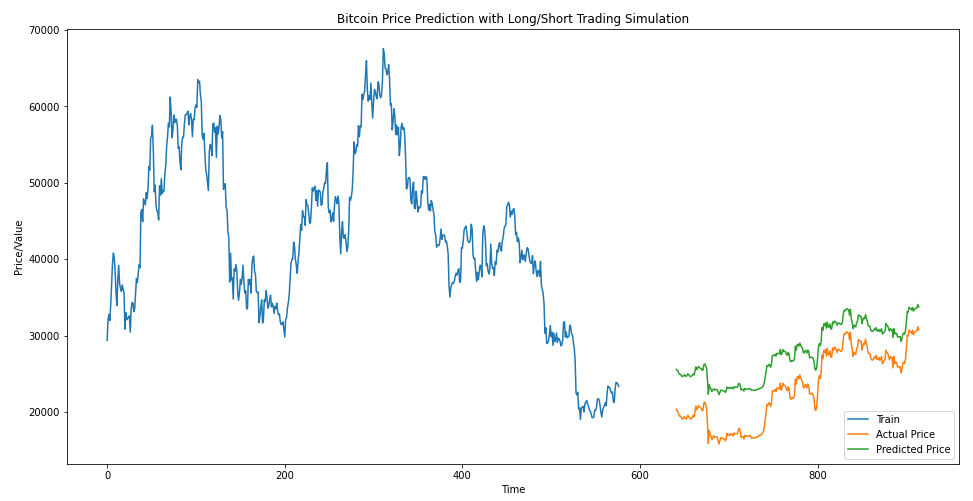
\includegraphics[scale=0.65]{fig10.jpg}
\caption{Bitcoin Price Prediction with Long/Short Trading Simulation }
\label{Bitcoin Price Prediction with Long/Short Trading Simulation }
\end{figure}

Figure 4.6 shows a comparison graph between the model's predictions and the actual prices of Bitcoin. Understanding the model's adherence to actual price movements is made easier thanks to this visualization.

\subsection{LSTM Model With Adjusted (No of Days)}

\begin{enumerate}
    \item \textbf{Import Necessary Libraries:}
\end{enumerate}

Libraries for managing data (numpy and pandas), preparing data (MinMaxScaler), creating models (keras LSTM model), and visualizing data (matplotlib) are all imported.

\textbf{2. Data Loading and Preprocessing:}

A data frame called df is filled with Bitcoin price information.

Datetime formatting is applied to the Date column.

The date is used to order the data.

The daily \% change in closing prices is calculated and stored in a new column called Return.

\textbf{3. Data Normalization:}

Only the Close prices—which are kept in new data—are taken into account for modeling.

The closing prices are then normalized (scaled) with MinMaxScaler, a typical preprocessing step for neural networks so that they lie between 0 and 1.

 \textbf{4. LSTM Model Definition:}
To create an LSTM model, a function called create lstm model() is defined. A Dense layer with one unit (for price prediction) follows two LSTM layers with 50 units each in the model.
The model is optimized with the Adam optimizer and utilizes mean squared error as its loss function.

\textbf{5. Splitting the training data:}

The training data is chosen over num days, a predetermined number of days. The remaining data is taken into account for validation.
X train (training) and X valid (validation) sets of the data have been created.

\textbf{6. Model Education:}

With a batch size of 1, the LSTM model is trained on the training data (X train) for 10 epochs.

\textbf{7. Making Predictions}

On the validation data (X valid), predictions are made using the trained LSTM model.
The inverse transformation of MinMaxScaler is then used to change these scaled forecasts back to the original pricing scale.

\textbf{8. Trading Strategy Implementation}

It uses a "long or short" trading approach. A long position is taken (i.e., the model predicts the price will climb) if the forecasted price for the following day is higher than the closing price of the current day. A short position is taken (i.e., the model forecasts the price will decline) if the projection is lower.

Based on the actual price change the following day, the capital is modified. If the price rises, the capital for a long position rises, and if the price falls, the capital for a short position rises.



\textbf{9. Visual Representation:} 

- To show the performance of the model, a graphical representation is made.

- The actual closing prices, the anticipated prices, and the data set intended for training are shown in the graph.

- The effectiveness of the trading technique and the model's alignment of forecast with real price are both revealed by this visualization. 

We can edit the No of days as shown in the figure below and the output will be generated with the portfolio value 

\begin{figure}[H]
\centering
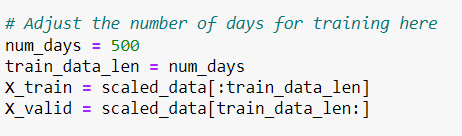
\includegraphics[scale=0.65]{fig15.jpg}
\end{figure}

Below Visualisation is selected in 14 days.

\begin{figure}[H]
\centering
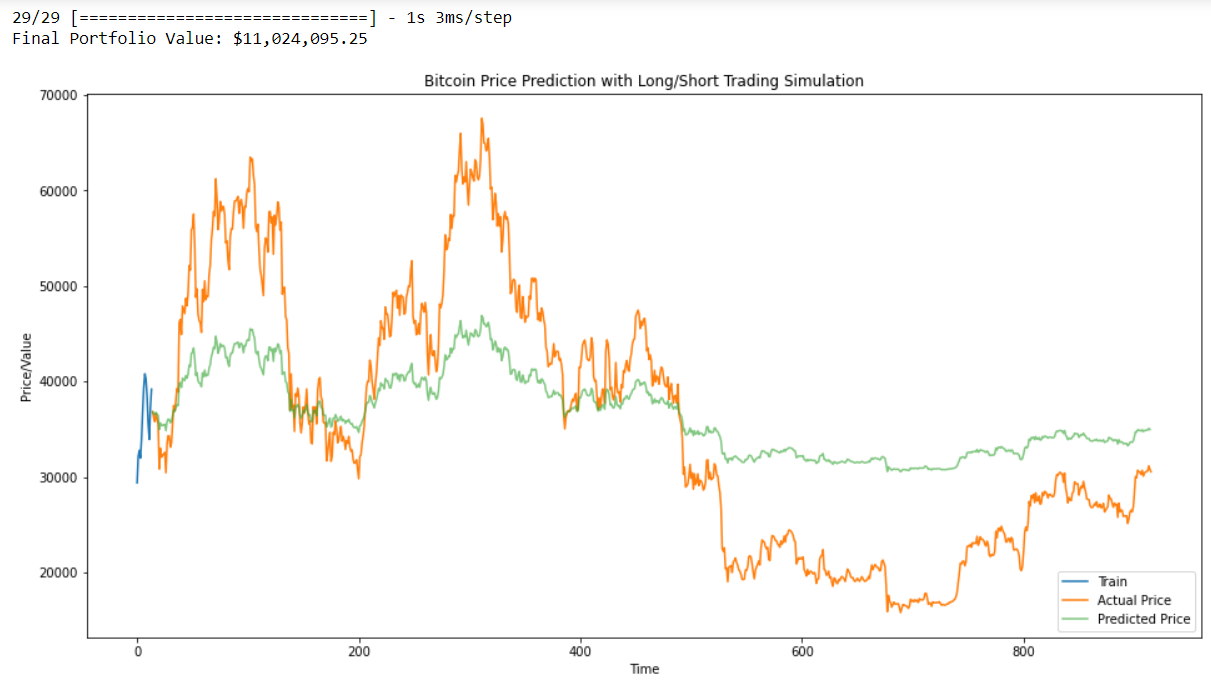
\includegraphics[scale=0.65]{fig11.jpg}
\caption{Adjust the number of days for training(14 Days)}
\label{Adjust the number of days for training}
\end{figure}

Below Visualisation is selected in 30 days.

\begin{figure}[H]
\centering
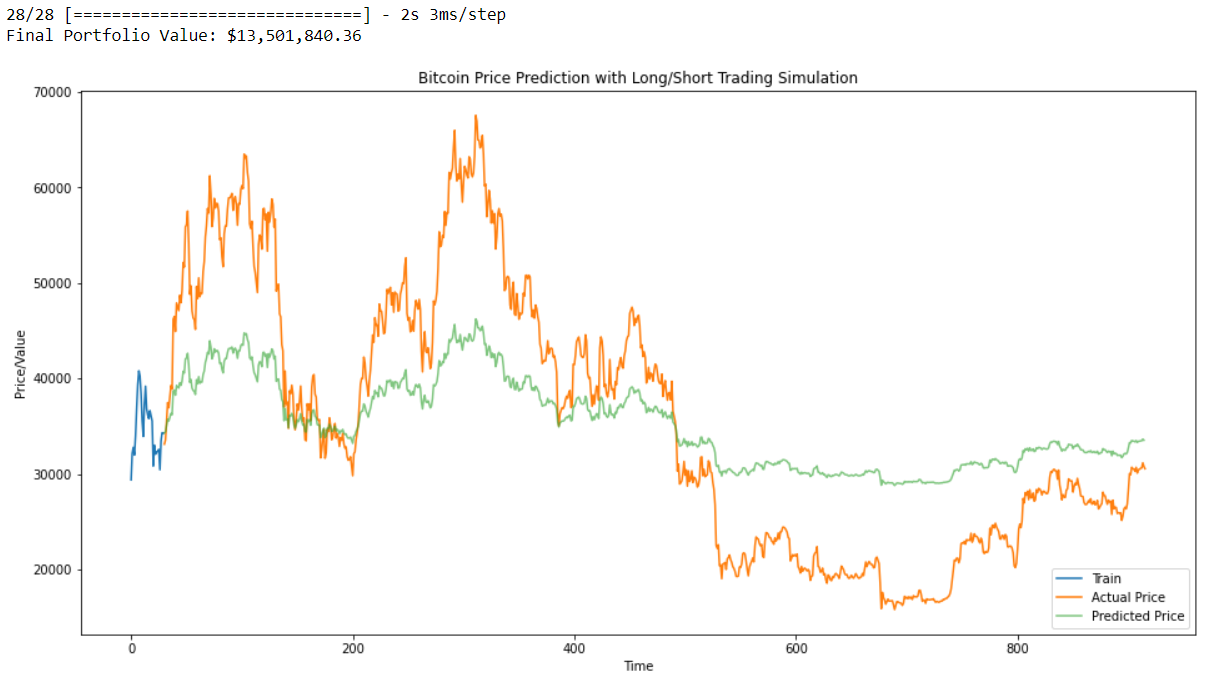
\includegraphics[scale=0.65]{fig12.jpg}
\caption{Adjust the number of days for training(30 Days)}
\label{Adjust the number of days for training}
\end{figure}

Below Visualisation is selected in 90 days.

\begin{figure}[H]
\centering
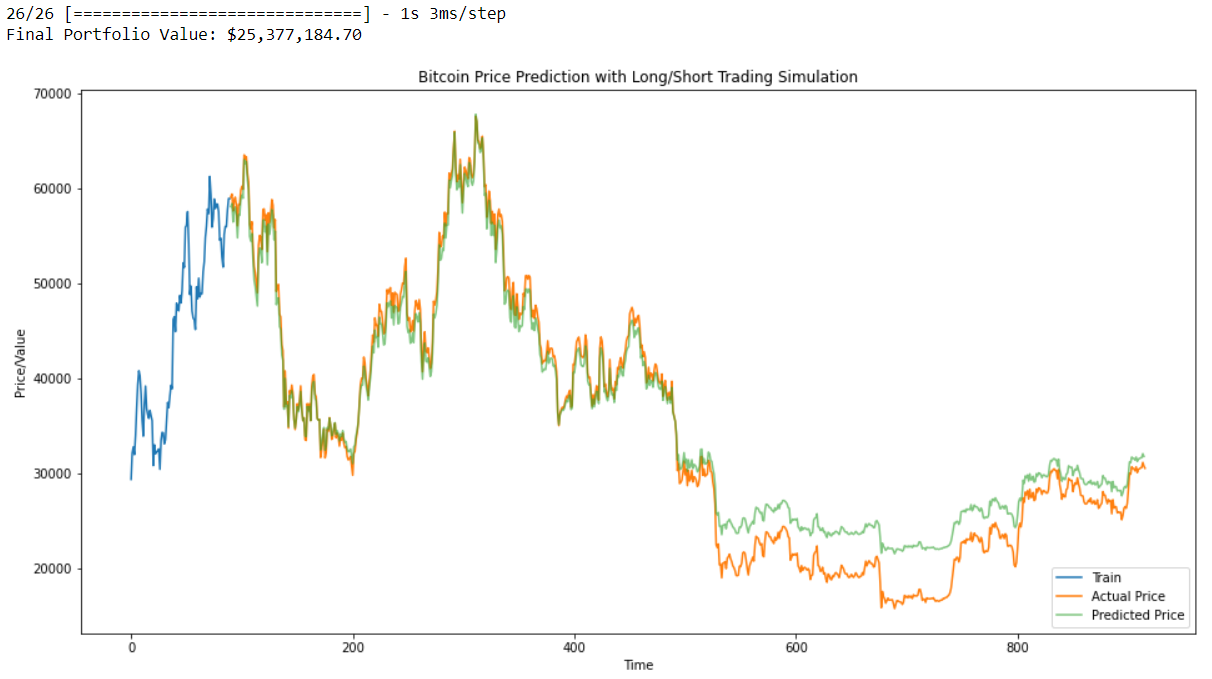
\includegraphics[scale=0.65]{fig13.jpg}
\caption{Adjust the number of days for training(90 Days)}
\label{Adjust the number of days for training}
\end{figure}

Below Visualisation is selected in 300 days.

\begin{figure}[H]
\centering
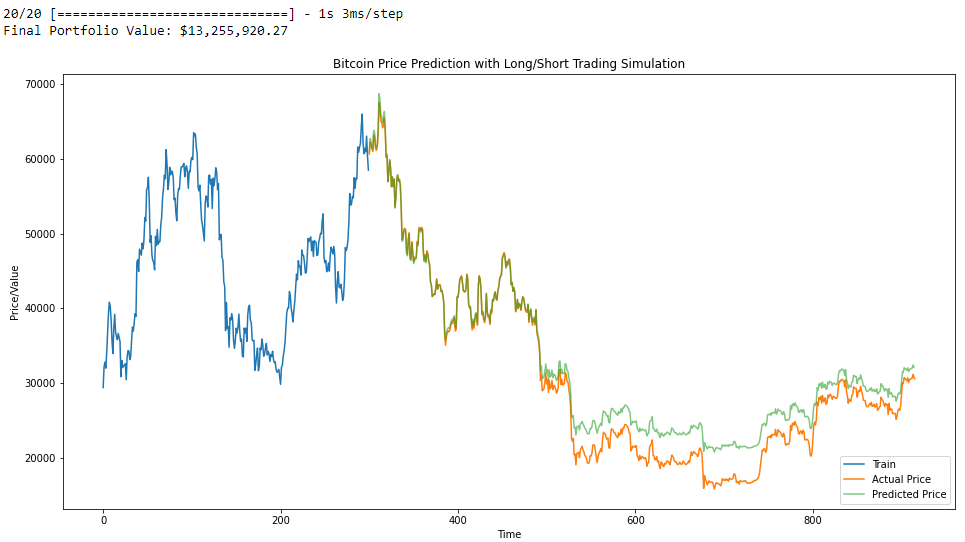
\includegraphics[scale=0.65]{fig14.jpg}
\caption{Adjust the number of days for training(300 Days)}
\label{Adjust the number of days for training}
\end{figure}



\subsection{Conclusion for LSTM Performance:}

The LSTM model has demonstrated its effectiveness in predicting changes in the price of Bitcoin. The model's flexibility when applied to various training window widths and the significant profits made, particularly with a 90 percent training window, highlight its promise for financial forecasting. However, because cryptocurrency markets are inherently unpredictable, it is important to utilize this model's predictions carefully, as with all others.

\section{Comparative Analysis:}

This study conducted a comparative examination of two well-known models, the Random Forest, and the LSTM neural network, in order to gauge the effectiveness of machine learning models in forecasting changes in the price of bitcoin.

\textbf{1.	Model complexity and training time:}

-	 \textbf{Random Forest:} It is a multi-decision tree ensemble learning technique with a relatively complex structure. In contrast to deep learning models, nevertheless, its parallel processing power frequently leads to shorter training times.

-	\textbf{LSTM:} Due to their numerous layers and recurrent structure, LSTM networks are typically computationally demanding. Particularly with larger datasets, they typically take longer to train.

\textbf{2.	Feature Interpretability:}

-	\textbf{Random Forest:} The capability of Random Forest to rate the importance of traits is one of its strengths. This can help with model interpretation and future feature engineering by revealing which features (or variables) are responsible for the predictions.

-	\textbf{LSTM:} Because they are a particular kind of neural network, LSTMs do not naturally provide the same level of feature interpretability as Random Forest. Although there are ways to analyze deep learning models, they are frequently more complicated and might not offer as many insightful details.

\textbf{3. Performance Metrics:}

-	\textbf{ Random Forest:} model demonstrated admirable performance metrics over a range of training and validation periods. It regularly made money and displayed flexibility across various data segments.

-	\textbf{LSTM:} The LSTM model produced a sizable return, especially when trained with a 90 percent window size, demonstrating its promise for financial forecasting. However, with various hyperparameter values or training methods, its performance could vary more noticeably.

\textbf{4.	Economic Implications: }

-   \textbf{Random Forest:} The model's forecasts were translated into a trading strategy that produced large gains, highlighting the model's usefulness for Bitcoin trading.

-   \textbf{LSTM:} The "long or short" trading strategy based on LSTM's predictions on the test data also generated significant gains, highlighting the importance of LSTM from an economic standpoint for Bitcoin trading.

\textbf{5.	Adaptability to New Data:}

-	\textbf{Random Forest:} Even though Random Forest can, in some cases, adapt to changes in data distribution, it may occasionally need retraining or fine-tuning, particularly in extremely volatile markets like cryptocurrency.

-	\textbf{LSTM:} LSTM networks may be better equipped to adapt to the changing nature of financial data because they are built to capture long-term dependencies in sequences. However, in order for them to efficiently recognize new patterns, they may also need retraining on occasion.

\subsection{Conclusion for Comparative Analysis:}

Both the Random Forest and LSTM models have demonstrated their abilities to forecast the course of the Bitcoin price. Long-term temporal patterns are better captured by LSTM networks than by Random Forest, which also may offer faster training times. The decision between the two should take into account the task's specific needs, the computational resources at hand, and how much weight is given to model interpretability. Both models have demonstrated their value in the context of this study, each providing particular advantages in the field of cryptocurrency price prediction.

\section{Summary of the Results}

In this chapter, We looked closely at the outcomes of using the two cutting-edge machine learning algorithms Random Forest and LSTM to forecast changes in the price of bitcoin. The outcomes offer a thorough grasp of the possibilities and capabilities of these models in the complex and unpredictable realm of bitcoin trading. Here is a brief summary:

\textbf{1.	Random Forest Performance:}

-	Time Series Cross-Validation (TSCV) was used to test the ensemble model, which is known for combining several decision trees, throughout a range of training-validation windows.

-	Using performance indicators like RMSE, Accuracy, Precision, Recall, and F1-Score, it was possible to see how well it performed across various data segments in terms of prediction.

-	The significant profits made after turning the Random Forest model's forecasts into a workable trading strategy served to highlight the model's economic importance.

\textbf{2.	LSTM Performance:}

-	The sequential character of the Bitcoin prices was captured using the LSTM, a sort of recurrent neural network.

-	To determine the ideal window size, the model was trained on historical data of varied lengths. The model's capacity to predict prices in light of the quantity of previous data to which it was exposed improved with each iteration.

-	The LSTM model's predictions were translated to a "long or short" trading strategy, similar to the Random Forest model, and the economic results were evaluated.

\textbf{3.	Comparative Analysis:}

-	The two models were compared side by side to reveal their advantages and shortcomings.

-	Model complexity, training time, interpretability of features, performance measures, economic ramifications, and adaptability to new data were some of the factors covered, giving a comprehensive overview of how they apply to cryptocurrencies.

In essence, this chapter emphasizes how machine learning and deep learning models have the ability to make sense of the frequently unexpected world of Bitcoin values. While both models demonstrated admirable performance, they each have distinct advantages, highlighting the need to match the model chosen to the particulars of the forecasting task and the particulars of the available data.


\def\baselinestretch{1.66}
\medskip

%%% ----------------------------------------------------------------------
%\include{Ch4} 
%\include{Ch5}
%\include{Ch6} 
% ......
% ------------------------------------------------------------------------
% -*-TeX-*- -*-Hard-*- Smart Wrapping
% ------------------------------------------------------------------------
\def\baselinestretch{1}

\chapter{Discussion}

\def\baselinestretch{1.44}

%%% ----------------------------------------------------------------------
The use of machine learning models to forecast the intricate changes in Bitcoin prices has revealed both opportunities and difficulties. This section aims to offer a thorough analysis of the results, taking into account both the advantages and disadvantages of our method.

\section{Interpretation of Findings}

\textbf{Model Distinctions:}

-	Multiple decision trees are used by the Random Forest model, an ensemble method, to create predictions. As non-linearities and interactions between characteristics are frequent in financial datasets, this model excels at capturing them (Breiman, 2001). The temporal dependencies, which are critical in time series data like Bitcoin prices, are not automatically taken into consideration.

-	On the other hand, the LSTM (extended Short-Term Memory) model, a kind of recurrent neural network, is especially suited for time series forecasting since it is explicitly built to recognize and recall across extended sequences \citep{Hochreiter1997LongSM}. It is a good option for our dataset because of its ability to retain previous information, which helps in capturing temporal trends.

\textbf{Performance metrics}

-	The performance of the models was quantified using metrics including RMSE, Accuracy, Precision, and Recall. Although both models produced fantastic results, it's important to assess them in light of the volatility of the Bitcoin market. High accuracy doesn't always convert into financial advantages, underscoring the significance of the chosen trading strategy \citep{bao2017deep}.

\textbf{Economic Implications}

-	The large profits made by both models demonstrate their applicability in the context of the current trading environment. For traders and investing algorithms, the LSTM's capacity to benefit from "long or short" strategies in particular may prove to be a priceless asset \citep{krauss2017deep}.

\textbf{Optimal Training Window}

-	The investigation of different training window sizes produced an unusual finding. The best window size for our dataset was determined to be 70 percent for the Random Forest model, contrary to what one might expect as more historical data is generally thought to result in better predictions. The dynamic nature of financial time series data and the significance of model retraining to accommodate current developments are highlighted by this. \citep{baumeister2015sign}.

\textbf{Comparative Insights}

-	Although both models showed promise, they are ideal for various situations due to their individual strengths. The Random Forest can be useful for determining feature importance and for helping traders make wise judgments because of its interpretable properties. The LSTM, on the other hand, maybe more suitable for high-frequency trading given its deep learning capabilities, where the ability to spot minute patterns in data might result in significant profits. \citep{sirignano2019universal}.

\section{Implications in Bitcoin Trading}

-  When Bitcoin first appeared, the financial world was completely changed since it provided a decentralized alternative to established fiat currencies. The price of Bitcoin, the most well-known cryptocurrency, is regularly monitored, and its market dynamics are thoroughly examined. The use of machine learning to forecast Bitcoin price changes has broad repercussions, especially when using complex models like Random Forest and LSTM. Here is a look at how these computational approaches may have broader implications for the Bitcoin trading industry.

\textbf{Incorporation of External Factors }

-	\textbf{Holistic Market View:} Machine learning models can combine several datasets, allowing traders to take into account a variety of external factors in addition to previous pricing. Global economic events, geopolitical unrest, changes in the law, and technological developments in the blockchain industry could all fall under this category. The models can give traders a more thorough understanding of potential price drivers by analyzing such a large and diverse amount of data\citep{GANDAL201886}.

-	\textbf{Real-time Adaptability: }These models can be dynamically updated with fresh data because of this. The algorithms may update their forecasts as world events develop, preventing traders from being caught off guard by unexpected market changes sparked by outside events.

\textbf{Algorithmic Trading Strategies:}

-\textbf{	Reactive Algorithms:} Trading algorithms can be improved by predictive models, making them more receptive to changes in the market that occur in real-time. With such flexibility, traders can quickly modify their methods to take advantage of fleeting market opportunities or avoid unexpected downturns \citep{DBLP:journals/cacm/TreleavenGL13}.

-	\textbf{Strategic Automation}: Trade execution can be automated by using machine learning's accuracy. Trading professionals can automate buy/sell choices, guaranteeing they never miss a profitable trading window, by defining predetermined conditions based on model outputs.

\textbf{Behavioral Analysis:}

-	\textbf{Sentiment Gauge}: In addition to using numerical data, machine learning models can comb the web and analyze a tonne of text from forums, social media, news stories, and other sources. This allows them to determine whether the general attitude towards Bitcoin is one of bullish exuberance or bearish pessimism\citep{kristoufek2015main}.

-	\textbf{Predictive Sentiment Analysis:} These algorithms can provide insights into the future by comparing previous price movements with sentiment data from the past. An increase in optimistic emotion, for instance, can signal to traders the impending price rebound.

\textbf{Diversification Strategies:}

-	\textbf{Correlation Insights:} Machine learning techniques can clarify the complex connections between Bitcoin and other financial assets through correlation insights. Trading firms might more effectively diversify their portfolios, distributing risks and perhaps increasing returns, by identifying these relationships \citep{phillips2017predicting}.

-	\textbf{Asset Synergy:} Traders can carefully pair their investments to protect themselves against possible losses, for instance, if it is discovered that Bitcoin has an inverse relationship with a certain stock or commodity.

\textbf{Scalability:}

-	\textbf{Efficiency in Data Processing:} Processing large datasets quickly and effectively is one of machine learning's main advantages. This scalability guarantees that traders always have the most recent information at their fingertips in the fast-paced world of Bitcoin trading, where data is continuously generated \citep{bao2017deep}.

-	\textbf{Worldwide Market Insights:} Because of its scalability, worldwide market data may also be integrated, guaranteeing that traders are educated by a global viewpoint as well as localized data.

\textbf{Cost Efficiency: }

-	\textbf{Improved Trade Timing:} Traders can time the execution of their trades more effectively with more accurate predictions. Due to their ability to avoid buying at high points or selling at low points, this can result in lower transaction costs \citep{hendershott2011does}.

-	\textbf{Strategic Order Placement: }In addition, traders can place limit or stop orders more wisely with knowledge of expected price fluctuations, resulting in more favorable trade executions.

\textbf{Enhanced Security}

-	\textbf{Fraud detection:} Improving transactional security can be facilitated by machine learning. These models can swiftly identify abnormalities, including recognizing fraudulent activity or unauthorized access, by analyzing trends in transaction data \citep{bahnsen2015example}.

-	\textbf{Risk management}: Furthermore, by foreseeing probable market declines, traders can be informed to close their positions or set stop-loss orders, protecting their investments from significant losses.

\section{Drawbacks of the Study:}

No matter how carefully planned and carried out, every thorough study has certain inherent limits. The effort to use machine learning methods like Random Forest and LSTM to forecast changes in the price of Bitcoin is not an anomaly. Here, we list and explore the main drawbacks of this study:

\textbf{1. Historical Data Dependence:}

\textbf{Relevance Over Time:} Making forecasts primarily based on historical data implies that past trends will continue into the future. The usefulness of historical data is ephemeral because of the myriad of dynamic factors that affect financial markets, including cryptocurrency \citep{tay2001application}.

\textbf{Overfitting Concerns:} Complex machine learning models, like LSTM, may occasionally "overfit" to the data, capturing noise rather than the underlying trend. The model's performance on unobserved data may suffer from such overfitting \citep{DBLP:journals/jcisd/HawkinsBM03}.

\textbf{2. Exclusion of Exogenous Factors:}

\textbf{Limited Scope of Data:} Since the study's primary focus was on price data, it may have overlooked other effects that could have had a large impact on Bitcoin pricing, such as regulatory changes, technological improvements, or macroeconomic considerations \citep{bouri_hedge_2017}.

\textbf{Sentiment Analysis:} The mood expressed in news stories, on social media, or by well-known people can have a big impact on the price of Bitcoin. The inability to capture abrupt market feelings due to the omission of such sentiment data can be a drawback \citep{kristoufek2015main}.

\textbf{3. Model Complexity:}

\textbf{Computing Demand:} Particularly with deep learning models like LSTM, there may be significant computational requirements that call for specialized hardware and may make real-time predictions difficult \citep{Goodfellow-et-al-2016}.

\textbf{Interpretability:} Models like Random Forest and LSTM are sometimes referred to as "black boxes," meaning that it is unclear how they operate inside and how they make decisions. This lack of openness among traders may impede trust and broader adoption \citep{DBLP:conf/kdd/Ribeiro0G16}.

\textbf{4. Market Dynamics:}

\textbf{High Volatility:} Bitcoin and other cryptocurrencies in particular are infamously unstable. Unpredictable variables, including rapid market panics or irrational exuberance, can be the cause of this volatility \citep{GANDAL201886}.

\textbf{Manipulative Activities:} Practices like "pump and dump" strategies have the potential to unpredictable skew price movements. Models may be misled by such manipulative strategies, particularly if the training data includes instances of market manipulation \citep{griffin2020bitcoin}.

\textbf{5. Generalizability Concerns:}

\textbf{Asset Specificity:} Although the study concentrated on Bitcoin, its conclusions could not be directly transferable to other cryptocurrencies or financial assets due to different market dynamics \citep{corbet2018bitcoin}.

\textbf{Temporal Limitations:} The time period selected for data collection may not have included all important developments affecting Bitcoin prices. According to \cite{bao2017deep}, models that have been trained on specific time frames may not generalize well to future periods with different market conditions.
% ------------------------------------------------------------------------
% -*-TeX-*- -*-Hard-*- Smart Wrapping
% ------------------------------------------------------------------------
\def\baselinestretch{1}

\chapter{Conclusion}

\def\baselinestretch{1.66}

%%% ----------------------------------------------------------------------

 

%%% ----------------------------------------------------------------------
\goodbreak

%\bigskip

%%% ----------------------------------------------------------------------


\section{Summary:}
Bitcoin is at the forefront of the emerging cryptocurrency industry, which has experienced tremendous growth and volatility over the past ten years. The goal of this research was to forecast changes in the price of Bitcoin by using advanced machine-learning techniques, notably Random Forest and LSTM.

\textbf{Key Undertakings:}

Data Preparation: The study painstakingly selected a dataset, with special emphasis on Bitcoin's previous pricing. To make the data eligible for model intake, it underwent thorough preprocessing, scaling, and transformation \citep{needham2007primer}.

\textbf{Modelling and Evaluation:}

-	\textbf{Random Forest}: Random Forest, an ensemble learning method, proved skilled in identifying complex non-linear patterns in the data. The model's effectiveness in predicting the price trajectories of Bitcoin was shown by measures like \gls{rmse} and accuracy \citep{breiman_random_2001}.

-	\textbf{\gls{lstm}:} As a deep learning model with a focus on sequence data, \gls{lstm}demonstrated its aptitude for forecasting the temporal trends seen in Bitcoin price movements. The robustness of the model was shown by its capacity to adapt across various training windows \citep{Hochreiter1997LongSM}.

\textbf{Trading Implications:} The study went beyond purely academic curiosity by simulating trading strategies based on model forecasts. Given the dynamic nature of bitcoin trading, Random Forest and \gls{lstm} both facilitated trading methods that might potentially provide substantial gains \citep{kristoufek2015main}.

\textbf{Comparative Analysis:} Although both models performed admirably, they both had advantages and disadvantages that were clear when they were compared. Such information is priceless for potential stakeholders debating the adoption of a model \citep{bao2017deep}.

\section{Limitations and Future Directions:}

The study's empirical validity was maintained by acknowledging its inherent limitations. These restrictions also opened the door for potential new research directions, including the incorporation of sentiment analysis and the investigation of additional sophisticated models \citep{bouri_hedge_2017}.

\textbf{1. Historical Data:} Although history frequently repeats itself, past performance is not always a reliable predictor of future outcomes. This is because the prediction models are trained on historical data. \citep{DBLP:books/lib/HastieTF09}.

\textbf{2. External Factors:} A wide range of external factors, including the state of the global economy, governmental reforms, technology developments, and significant geopolitical events, can have an impact on bitcoin pricing. Trading data may not always include them.

\textbf{3. Black-Box Nature:} Deep Learning models, particularly LSTMs, are frequently referred to be ”black boxes,” which makes it difficult to completely analyze and comprehend their predictions.

\textbf{4. Computational Constraints:} like LSTMs, have large computing resource requirements. In some circumstances, this might reduce the complexity or volume of data that can be processed.

\textbf{5. Overfitting:} Although overfitting is prevented by processes in models like Random Forest and LSTM, there is still a chance that the models will overfit the training data, which will limit their capacity to generalize to new data. \citep{DBLP:books/lib/HastieTF09}.

\textbf{6. Data Source Bias:} The trading data may have bias depending on the data source, which could be a specific trading exchange. An exchange that primarily serves institutional investors, for instance, can display distinct trading patterns than one that primarily serves regular investors.

\textbf{7. Timeframe Constraint:} The results of the study might be particularly applicable to the particular timeframe of the data used. The model’s performance might change as the Bitcoin market changes.


In conclusion, there are opportunities and challenges in the erratic world of Bitcoin. This research has outlined methods that data-driven insights can help traders, investors, and researchers navigate the turbulent waters of the cryptocurrency markets by utilizing machine learning and deep learning approaches.




%%% ----------------------------------------------------------------------
\goodbreak
\section{Future Work and Recommendations:}

The financial markets' dynamic nature and the cryptocurrency industry's constant evolution make it necessary to conduct continuing studies and improve forecasting models. The following suggestions and directions for further research are put forth in light of the results of our study and current crypto-financial landscape trends:

\textbf{1.Integrate Alternative Data Sources:}

\textbf{Sentiment analysis:} The sentiment found in news stories, blogs, and social media sites, notably Twitter, can have an impact on how much Bitcoin costs. To improve forecasting accuracy, future research can concentrate on fusing sentiment analysis with price prediction models \citep{li2020survey}.

\textbf{Blockchain analytics:} By utilizing on-chain data, including transaction volumes, active addresses, and hash rates, it may be possible to gain a better understanding of the Bitcoin ecosystem and increase the reliability of predictions \citep{cong2021tokenomics}.

\textbf{2.Advanced Model Architectures:}

\textbf{Hybrid models:} By combining the benefits of different models, such as \gls{lstm} and CNN or attention mechanisms, they may be able to predict outcomes more accurately \citep{chong2017deep}.

\textbf{Transfer Learning:} Models that have been previously trained on huge financial datasets and then fine-tuned using Bitcoin data can make use of general market trends to forecast Bitcoin-specific movements \citep{he2019transfer}.

\textbf{3.Portfolio Diversification:}

Future research should investigate how to combine Bitcoin with other assets to create diversified portfolios, given the inherent risk associated with cryptocurrencies. As a result, risk can be reduced and profits can be maximized \citep{guesmi2019portfolio}.

\textbf{4.Model Interpretability:}

Although models like the LSTM provide excellent accuracy, their "black-box" nature makes them difficult to interpret. According to \cite{DBLP:conf/kdd/Ribeiro0G16}, explainability research can increase stakeholders' trust and adoption.

\textbf{6.Real-time prediction System:}

For high-frequency trading and quick investment decisions, creating real-time forecasting systems, including live data streams, and instantly updating projections can be crucial \citep{xu2013emr}.

\textbf{5. Regulatory Considerations:}

Understanding and predicting the effects of future laws on Bitcoin prices can be a useful study avenue as governments and financial agencies around the world struggle to regulate cryptocurrencies \citep{zohar2015bitcoin}.

\textbf{6.Risk management:}

Future research should focus on creating risk management plans in addition to prediction models. This would guarantee that traders and investors may profit from opportunities while also protecting them from disastrous losses \citep{hull2012risk}.

As a result, even while the study that has been presented provides useful information on predicting the price of Bitcoin, there is still much to learn and improve due to the complexity and size of the field. The future of Bitcoin trading will be shaped by a synthesis of data science, finance, and subject expertise.

 

% ------------------------------------------------------------------------
\setlinespacing{1.44}
\bibliographystyle{agsm} % Use Harvard style 
%\bibliographystyle{apalike}
\bibliography{MyBib} % use your own bib file

%#### Include any appendix below #####
\appendix

% MATH -------------------------------------------------------------------
\newcommand{\A}{{\cal A}}
\newcommand{\h}{{\cal H}}
\newcommand{\s}{{\cal S}}
\newcommand{\W}{{\cal W}}
\newcommand{\BH}{\mathbf B(\cal H)}
\newcommand{\KH}{\cal  K(\cal H)}
\newcommand{\Real}{\mathbb R}
\newcommand{\Complex}{\mathbb C}
\newcommand{\Field}{\mathbb F}
\newcommand{\RPlus}{[0,\infty)}
%
\newcommand{\norm}[1]{\left\Vert#1\right\Vert}
\newcommand{\essnorm}[1]{\norm{#1}_{\text{\rm\normalshape ess}}}
\newcommand{\abs}[1]{\left\vert#1\right\vert}
\newcommand{\set}[1]{\left\{#1\right\}}
\newcommand{\seq}[1]{\left<#1\right>}
\newcommand{\eps}{\varepsilon}
\newcommand{\To}{\longrightarrow}
\newcommand{\RE}{\operatorname{Re}}
\newcommand{\IM}{\operatorname{Im}}
\newcommand{\Poly}{{\cal{P}}(E)}
\newcommand{\EssD}{{\cal{D}}}
% THEOREMS ---------------------------------------------------------------
\theoremstyle{plain}
\newtheorem{thm}{Theorem}[section]
\newtheorem{cor}[thm]{Corollary}
\newtheorem{lem}[thm]{Lemma}
\newtheorem{prop}[thm]{Proposition}

\theoremstyle{definition}
\newtheorem{defn}{Definition}[section]
%
\theoremstyle{remark}
\newtheorem{rem}{Remark}[section]
%
\def\baselinestretch{1}

\chapter{Appendix }

\def\baselinestretch{1.66}

\begin{figure}[H]
\centering
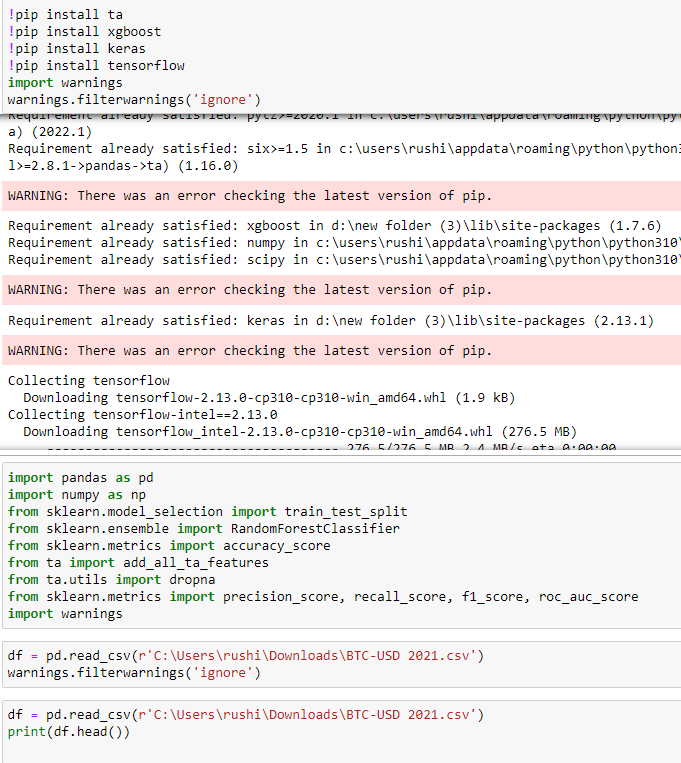
\includegraphics[scale=0.75]{fig16.jpg}

\end{figure}

\begin{figure}[H]
\centering
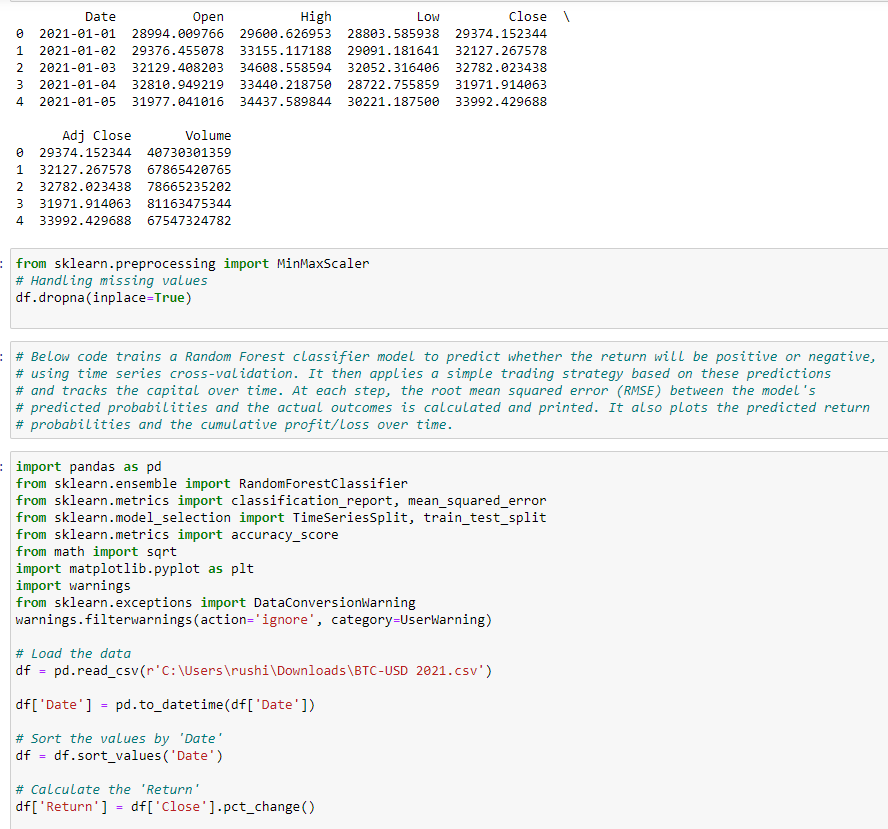
\includegraphics[scale=0.65]{fig17.jpg}
\end{figure}

\begin{figure}[H]
\centering
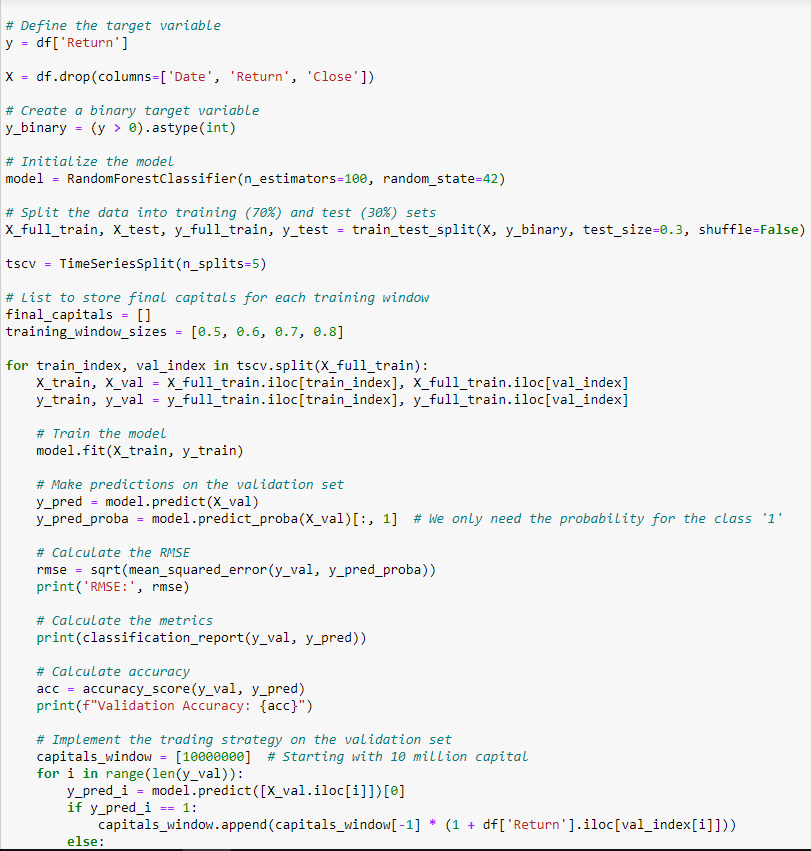
\includegraphics[scale=0.75]{fig18.jpg}

\end{figure}

\begin{figure}[H]
\centering
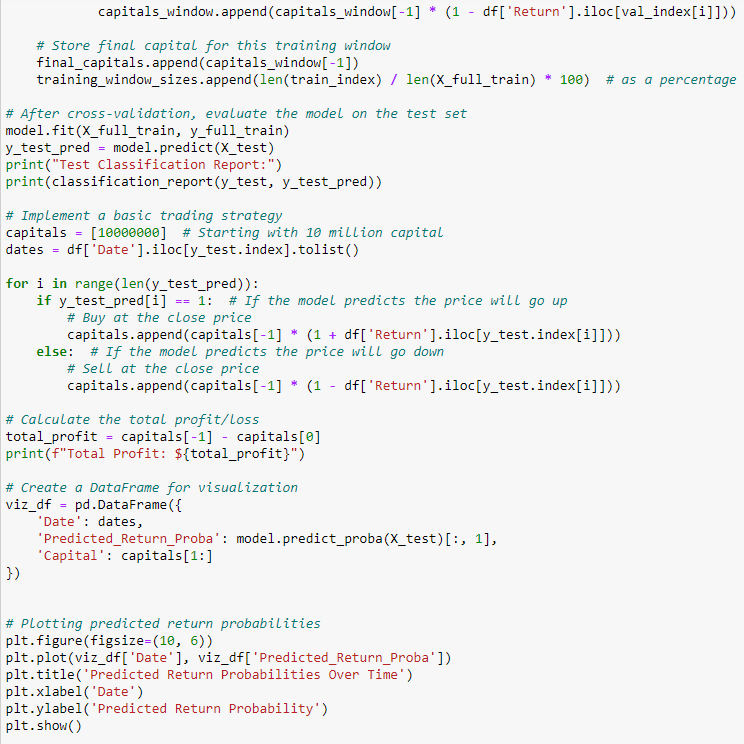
\includegraphics[scale=0.75]{fig19.jpg}

\end{figure}

\begin{figure}[H]
\centering
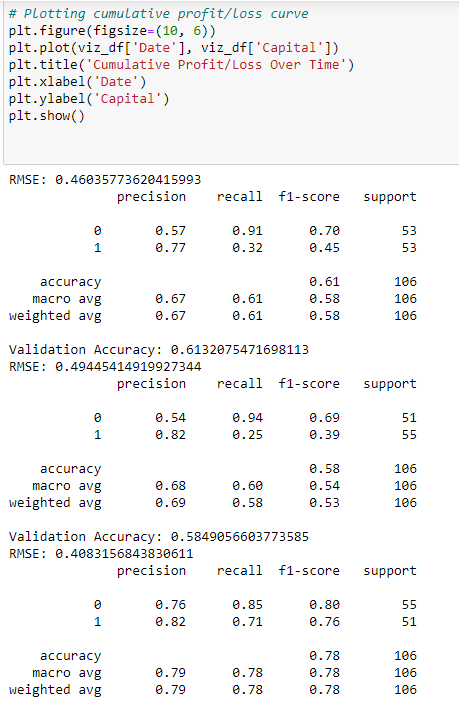
\includegraphics[scale=0.65]{fig20.jpg}
\end{figure}

\begin{figure}[H]
\centering
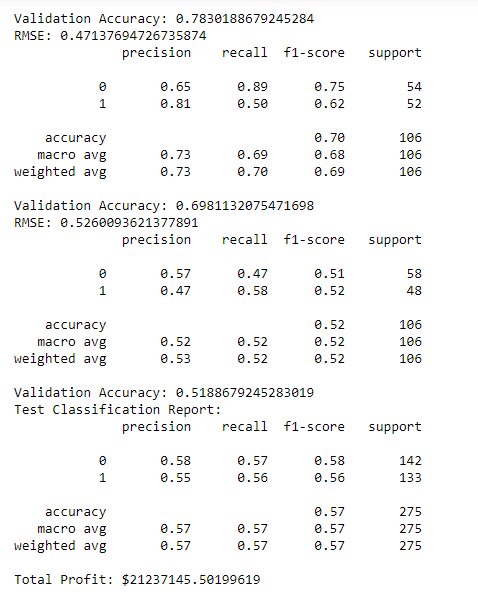
\includegraphics[scale=0.65]{fig21.jpg}
\end{figure}

\begin{figure}[H]
\centering
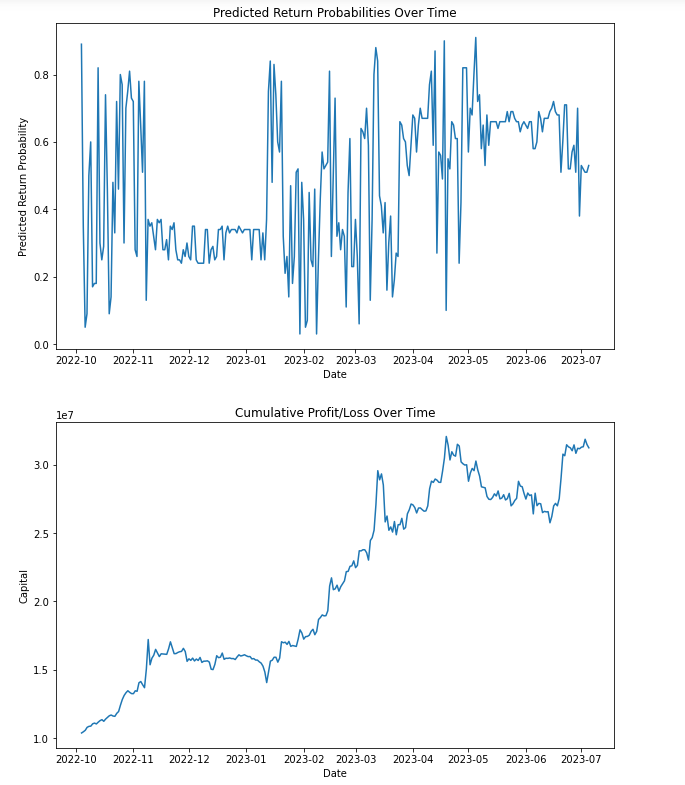
\includegraphics[scale=0.65]{fig22.jpg}
\end{figure}

\begin{figure}[H]
\centering
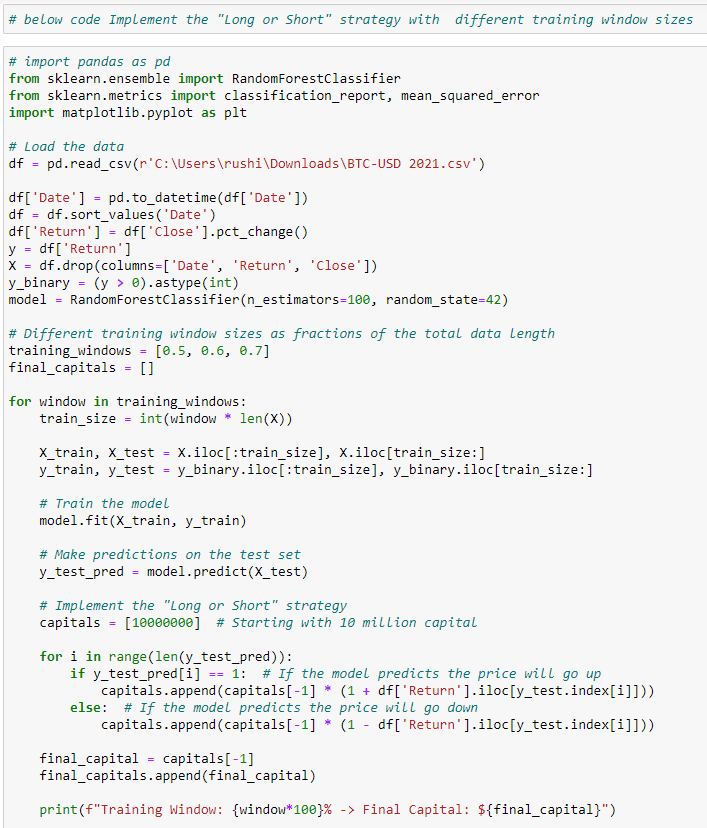
\includegraphics[scale=0.65]{fig23.jpg}
\end{figure}

\begin{figure}[H]
\centering
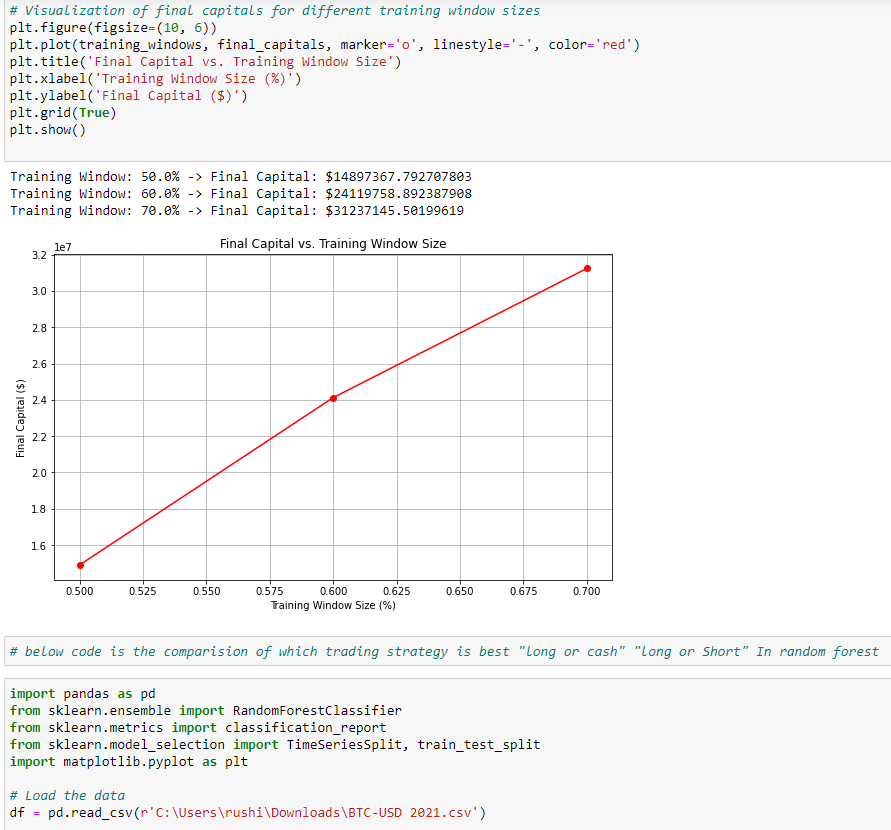
\includegraphics[scale=0.65]{fig24.jpg}
\end{figure}

\begin{figure}[H]
\centering
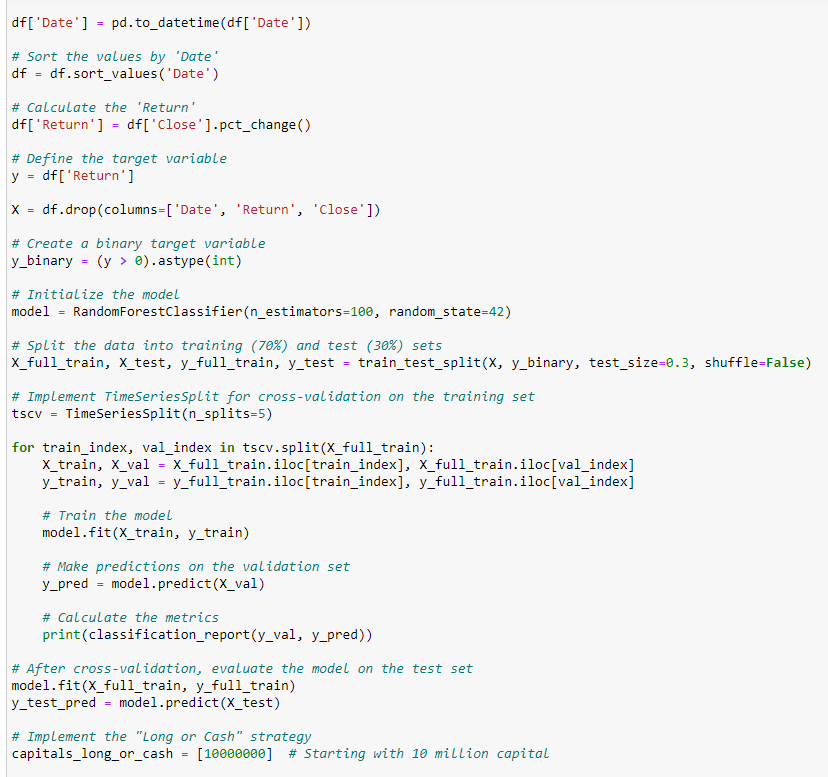
\includegraphics[scale=0.65]{fig25.jpg}
\end{figure}
\begin{figure}[H]
\centering
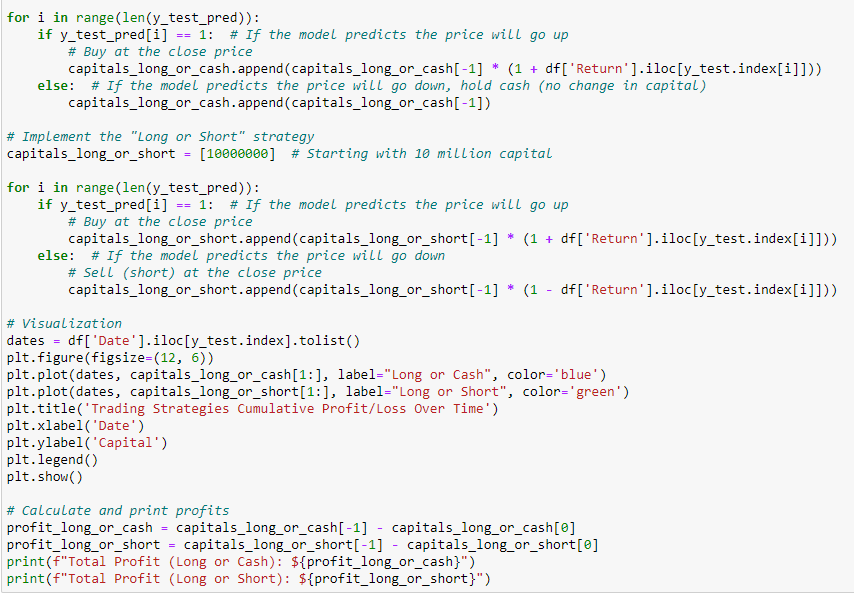
\includegraphics[scale=0.65]{fig26.jpg}
\end{figure}

\begin{figure}[H]
\centering
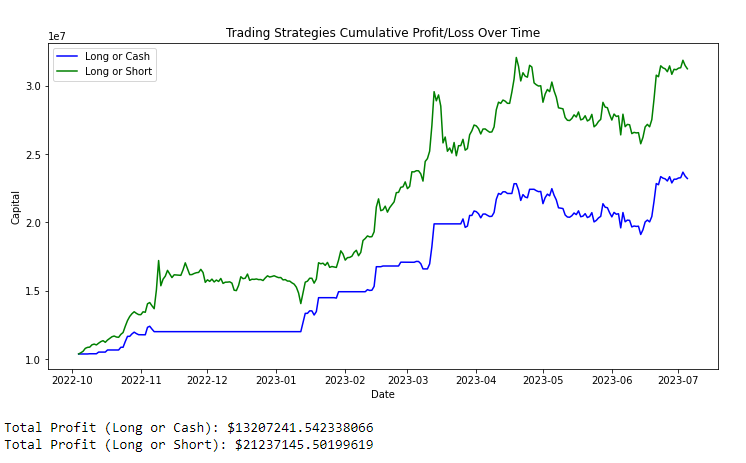
\includegraphics[scale=0.65]{fig27.jpg}
\end{figure}

\begin{figure}[H]
\centering
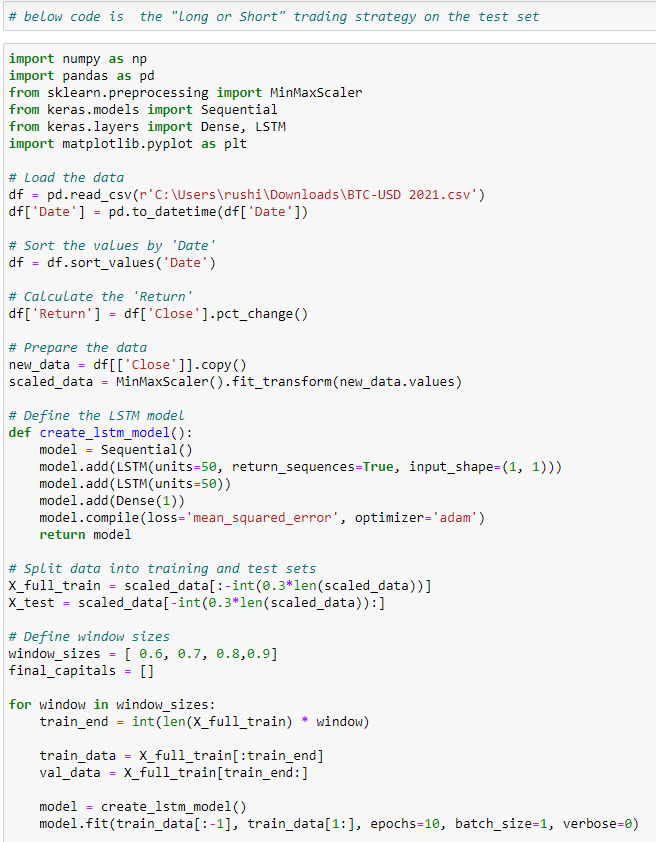
\includegraphics[scale=0.65]{fig28.jpg}
\end{figure}

\begin{figure}[H]
\centering
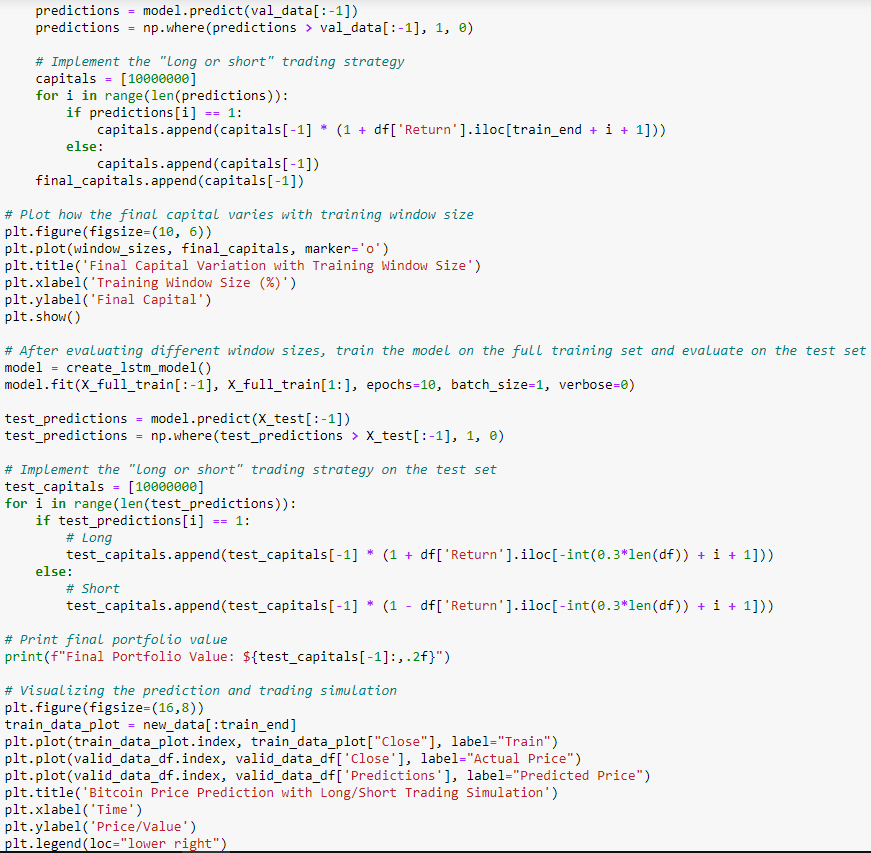
\includegraphics[scale=0.65]{fig29.jpg}
\end{figure}

\begin{figure}[H]
\centering
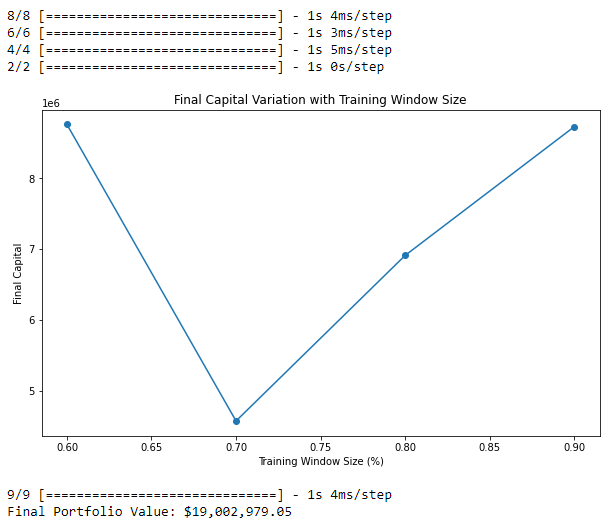
\includegraphics[scale=0.65]{fig30.jpg}
\end{figure}

\begin{figure}[H]
\centering
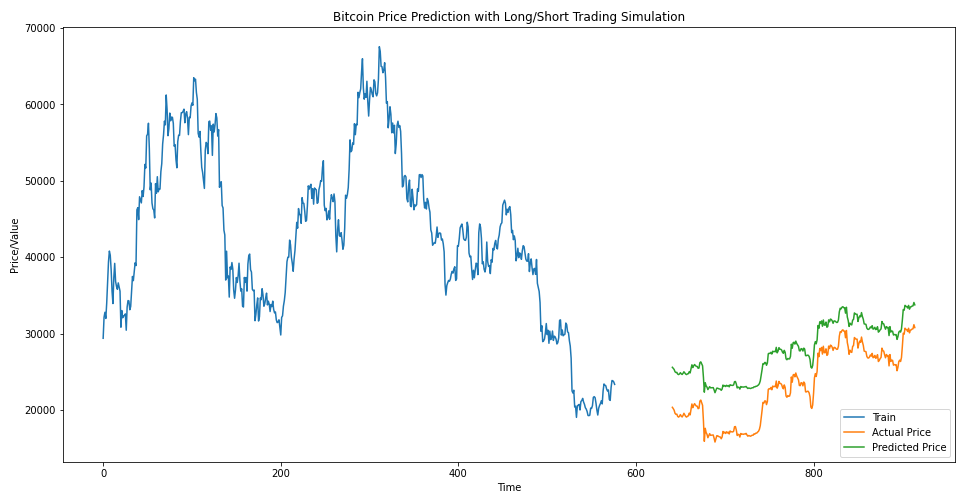
\includegraphics[scale=0.65]{fig31.jpg}
\end{figure}

\begin{figure}[H]
\centering
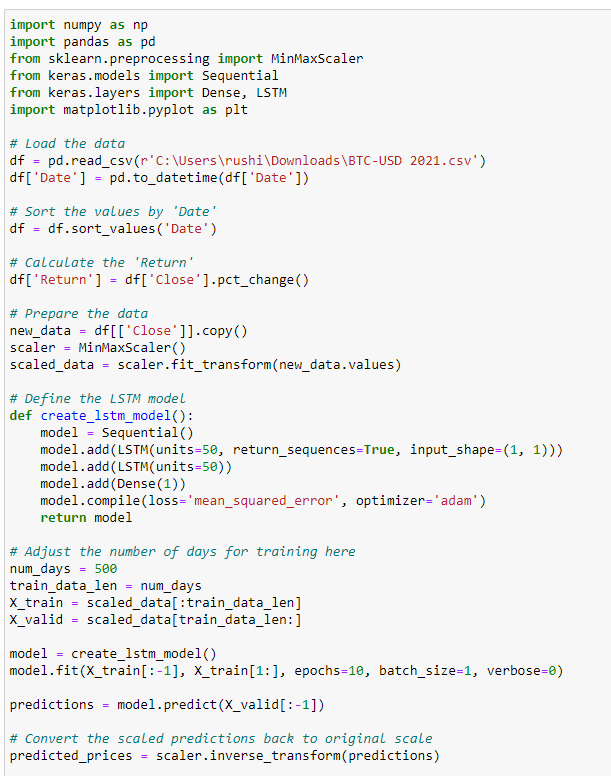
\includegraphics[scale=0.65]{fig32.jpg}
\end{figure}

\begin{figure}[H]
\centering
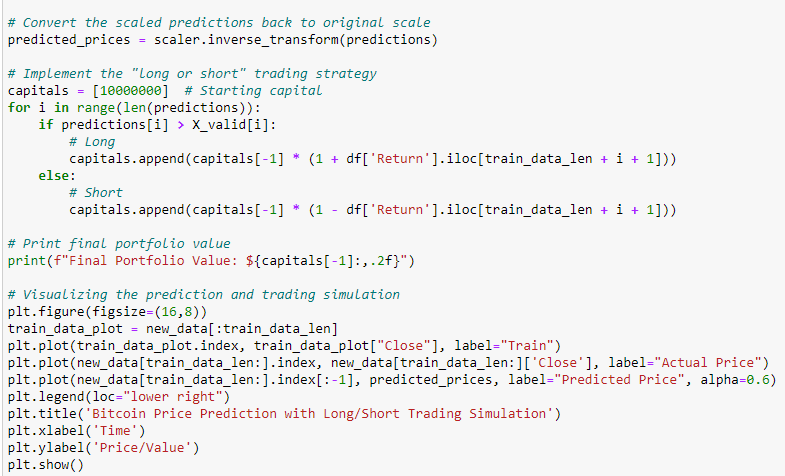
\includegraphics[scale=0.65]{fig33.jpg}
\end{figure}

\begin{figure}[H]
\centering
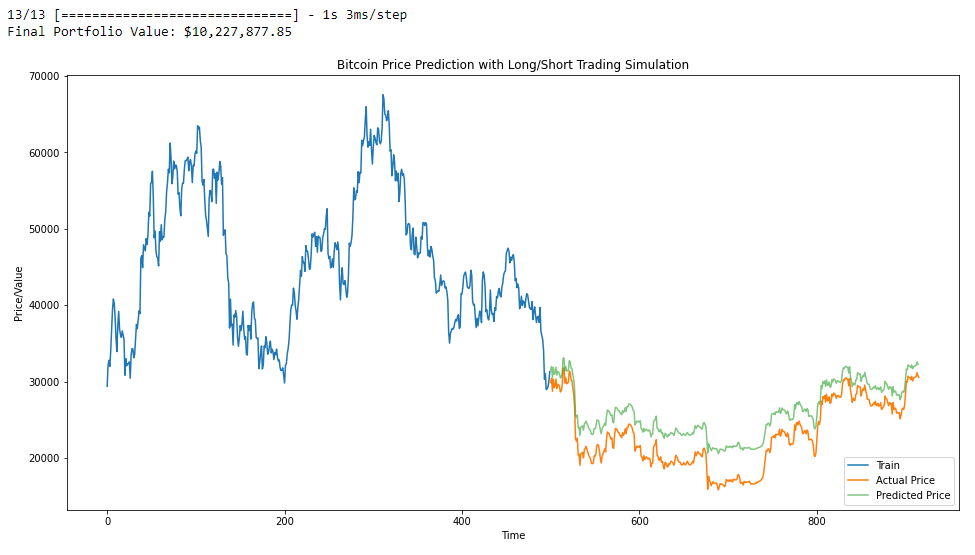
\includegraphics[scale=0.65]{fig34.jpg}
\end{figure}
 %\include{AppendixB}

% =================================================================
\end{document}
% ------------------------------------------------------------------------
